\documentclass{article}
\usepackage{graphicx}
\usepackage{listings}
\usepackage{float}
\usepackage{color}

\title{Tugas Pemrograman Chapter 2}
\author{Annisa Khairani(1184071) }
\date{29 October 2019}

\begin{document}

\maketitle

\section{Teori}
\subsection{Jenis-Jenis Variabel dan Cara Pemakaian Variabel }
\paragraph{}
    Variabel merupakan suatu wadah untuk menyimpan suatu data yang bersifat mutable yang artinya nilainya bisa diubah-ubah atau sementara, sedangkan data yang disimpan didalam variabel disebut dengan tipe data. Tipe Data tersebut terbagi menjadi beberapa macam, yaitu:
    \begin{enumerate}
        \item Tipe Data Angka
            \par Tipe ini terbagi menjadi beberapa jenis lagi, yaitu:
            \par \begin{enumerate}
                \item Integer (Bilangan Bulat), contohnya adalah 1,2,3,dst.
                \item Float (Bilangan Pecahan), contohnya adalah 1.5,2.1,3.1,dst.
                \begin{figure}[h]
                    \centerline{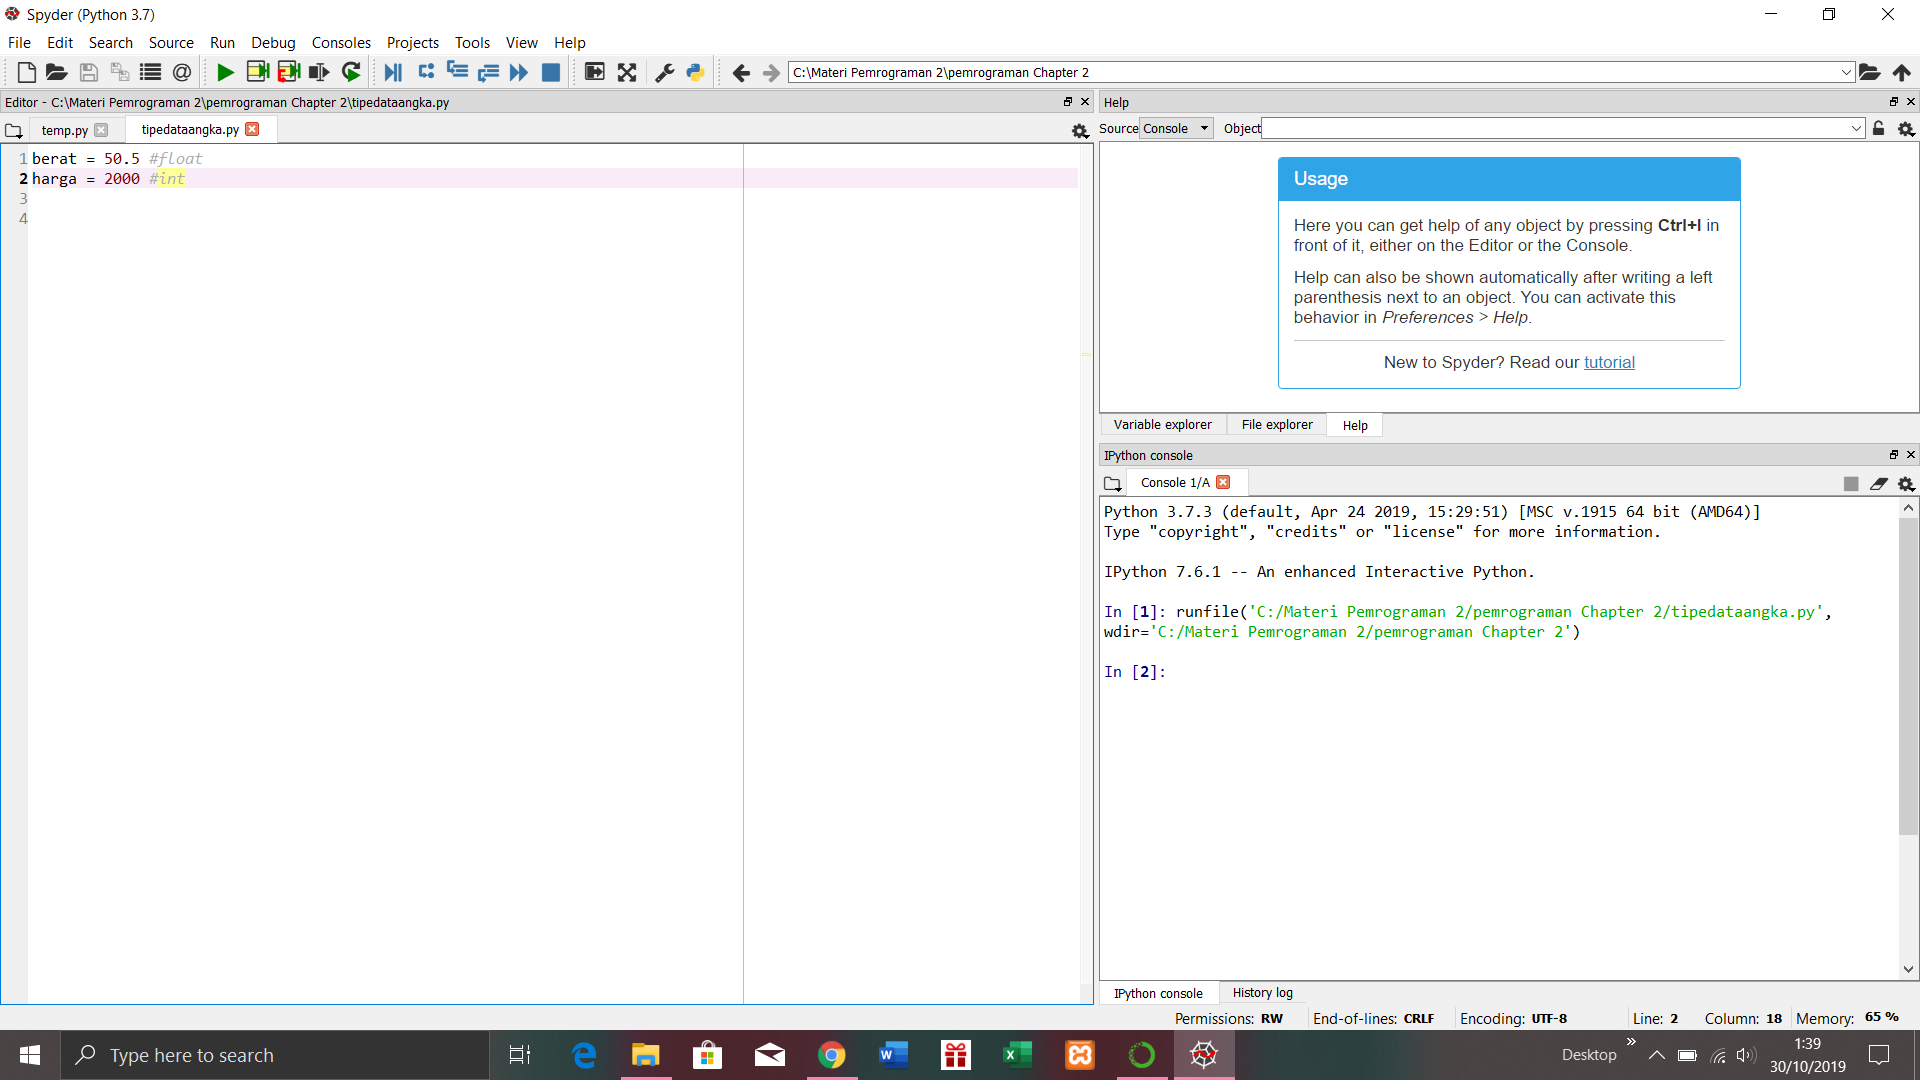
\includegraphics[width=8cm]{figures/tipedataangka.png}}
                \end{figure}
            \end{enumerate}
        \item Tipe Data Teks 
            \par Tipe ini terbagi menjadi dua jenis, yaitu:
            \par \begin{enumerate}
                \item String (Kumpulan Karakter), contohnya adalah "Saya sedang Tidur"
                \item Varchar (Karakter), contohnya adalah a,b,c,d,dst.
                \begin{figure}[h]
                \centerline{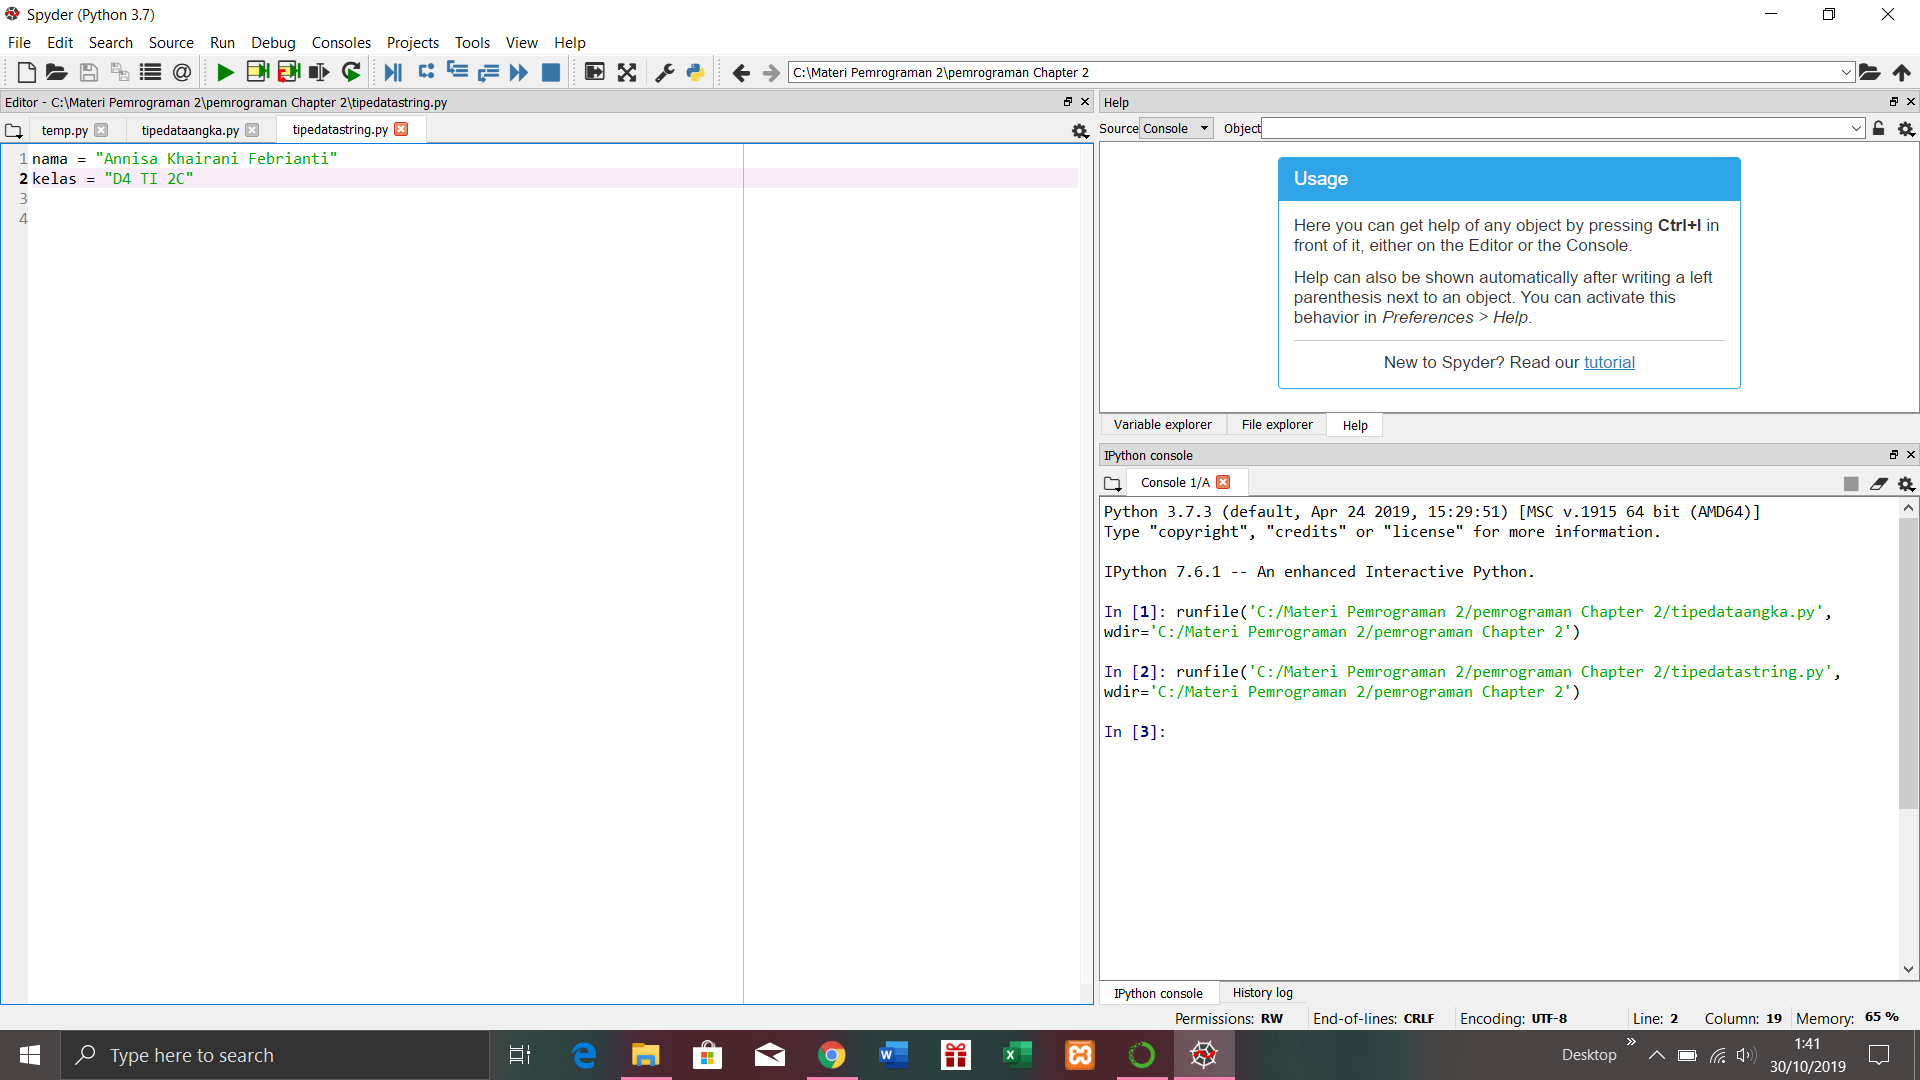
\includegraphics[width=8cm]{figures/tipedatastring.png}}
            \end{figure}
            \end{enumerate}
            \par Penulisan tipe ini harus diapit oleh tanda petik.
            \item Tipe Data Boolean
            \par Tipe data ini adalah tipe yang hanya memiliki dua nilai saja yaitu True dan False atau 0 dan 1.
            \begin{figure}[h]
                    \centerline{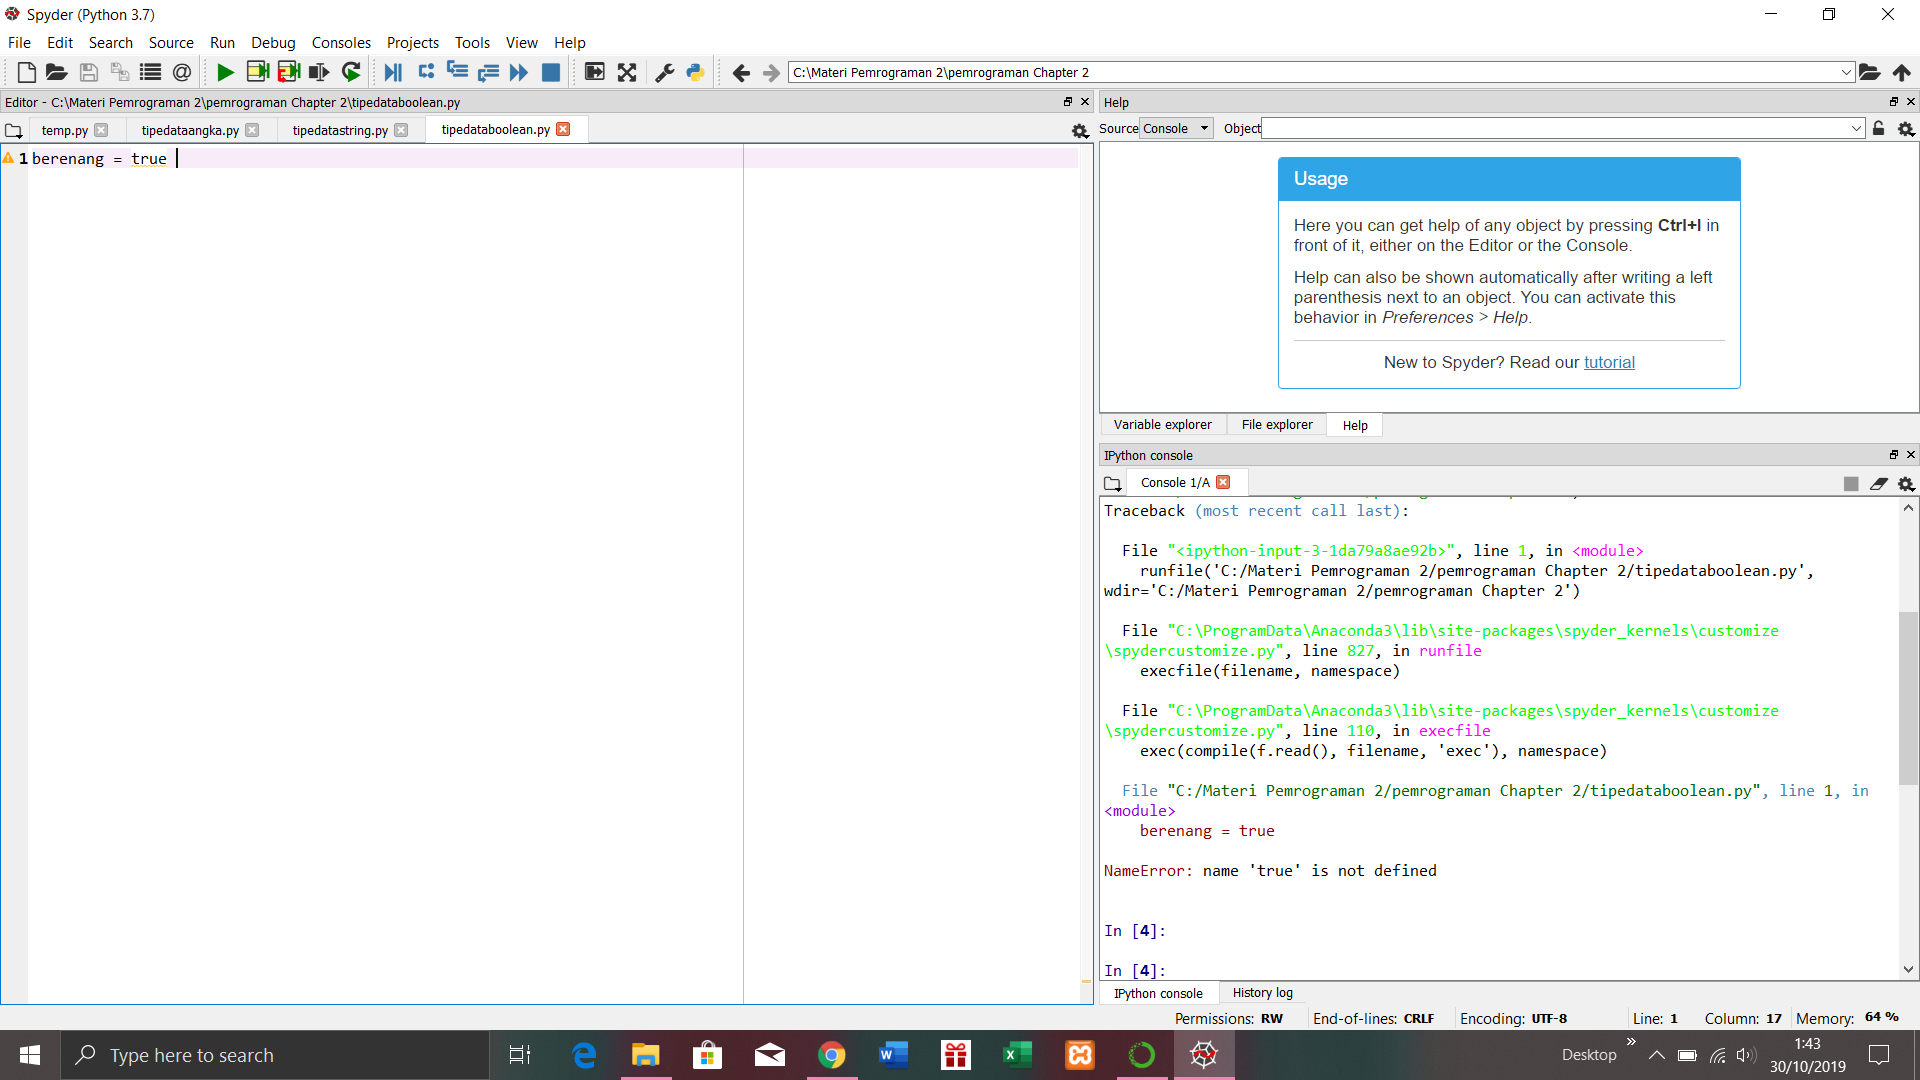
\includegraphics[width=8cm]{figures/tipedataboolean.png}}
            \end{figure}
    \end{enumerate}
\paragraph{} Adapun contoh penggunaan variabel menggunakan kode python adalah:
\paragraph{}
            \begin{figure}[H]
                \centering
                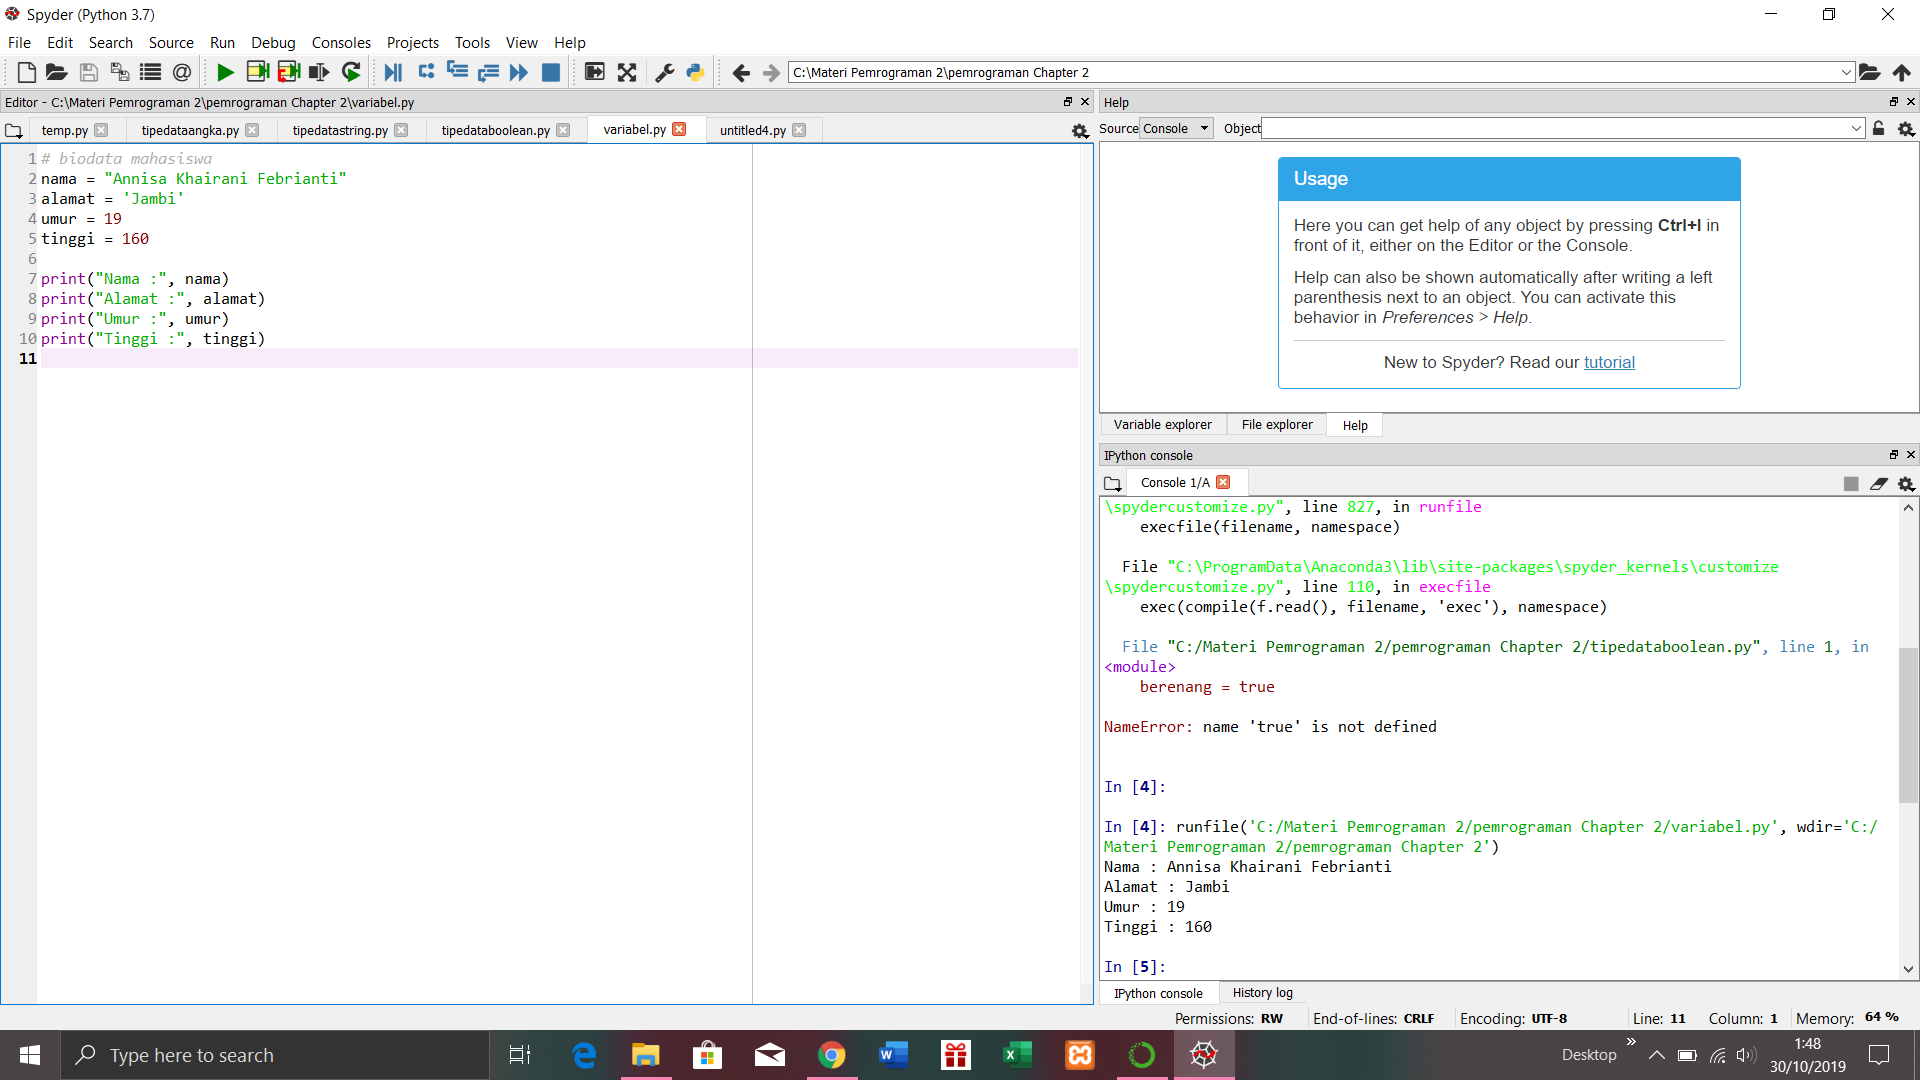
\includegraphics[width=8cm]{figures/variabel.png}
                \caption{Caption}
                \label{fig:my_label}
            \end{figure}
\lstinputlisting[language=Python]{figures/src/variabel.py}

\subsection{Kode Untuk Meminta Input Dari user dan Melakukan Output ke Layar}
\paragraph{} Input adalah suatu masukan yang akan kita berikan ke suatu program sedangkan hasil yang ditampilkan disebut dengan Output.
\begin{enumerate}
    \item Cara mengambil input
        \par Python menyediakan suatu fungsi input, dengan menggunakan kode input() 
    \item Cara menampilkan output
        \par Untuk menampilkan sebuah output teks kita menggunakan kode print()
\end{enumerate}
\begin{figure}[h]
                \centerline{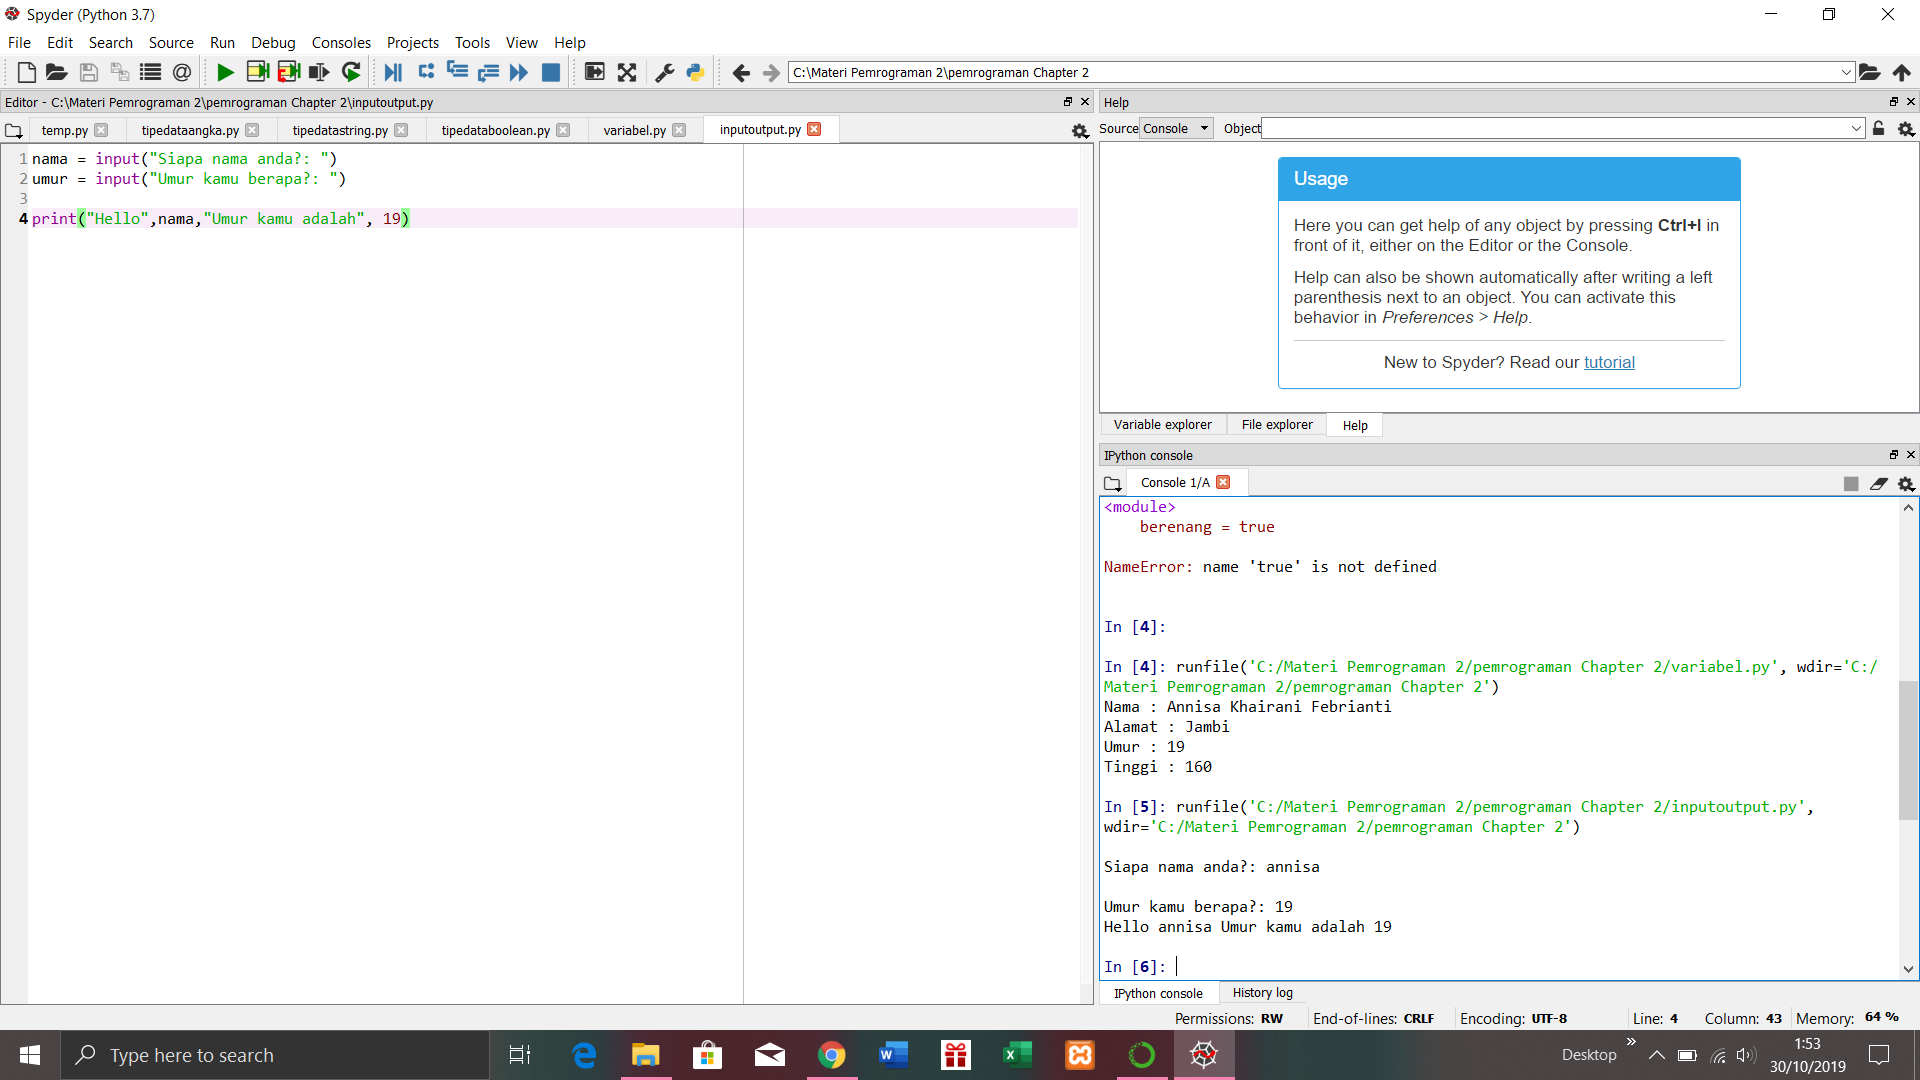
\includegraphics[width=8cm]{figures/inputoutput.png}}
\end{figure}
\lstinputlisting[language=Python]{figures/src/inputoutput.py}

\subsection{Operator Dasar Aritmatika, Tambah, Kali, Kurang, Bagi, dan bagaimana mengubah String ke Integer dan Integer ke String}
\paragraph{} Operator adalah suatu simbol yang digunakan untuk operasi tertentu. Dan operator aritmatika tersebut termasuk pada operator yang paling sering kita gunakan.
\paragraph{}
    \centerline{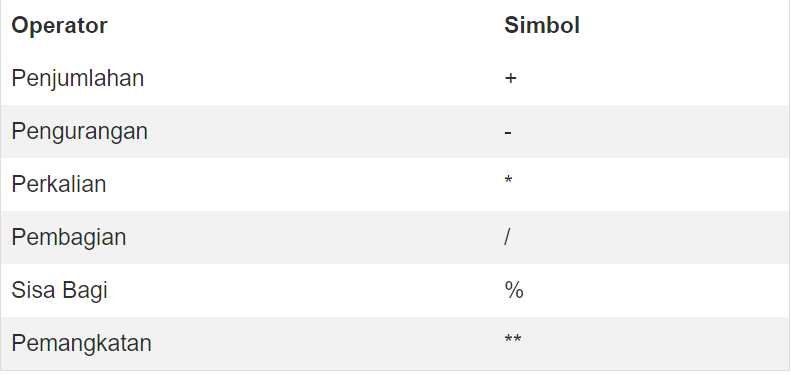
\includegraphics[width=8cm]{figures/operatoraritmetika.png}}
\paragraph{} Adapun contoh penggunaanya adalah:
\begin{figure}[h]
                \centerline{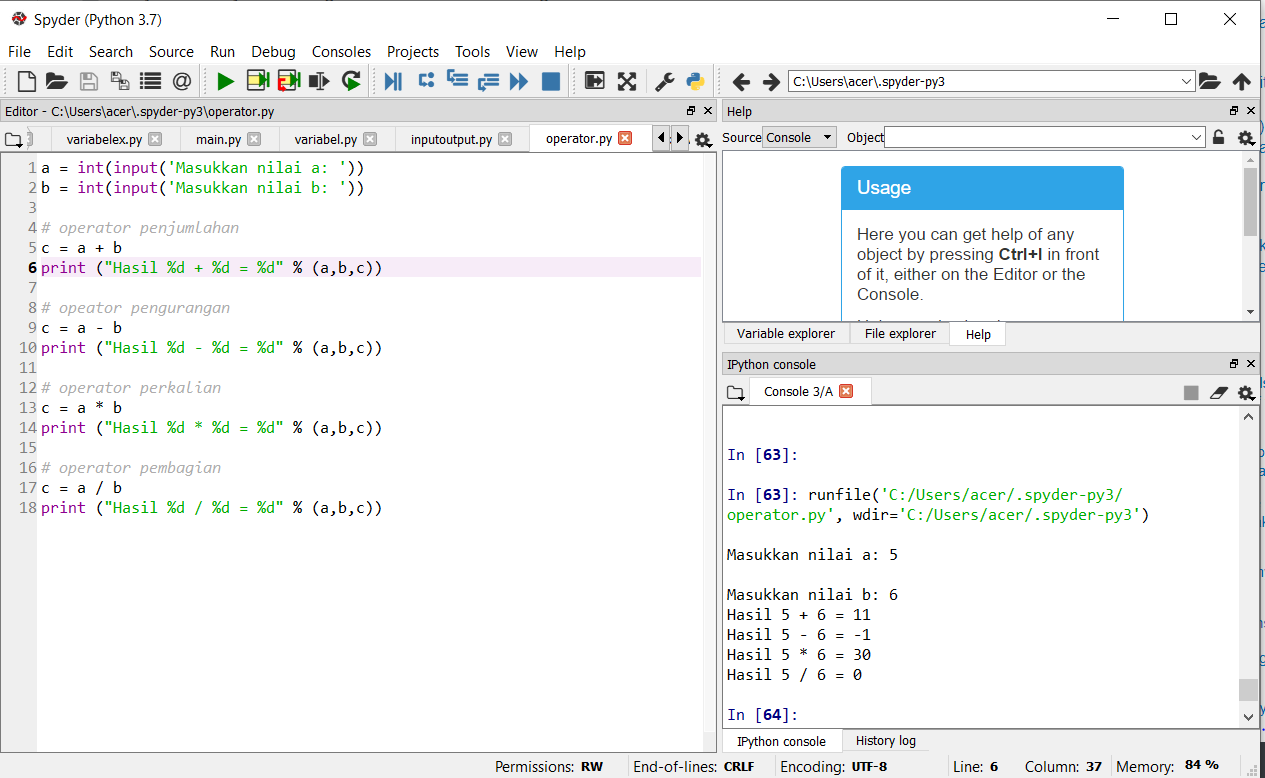
\includegraphics[width=8cm]{figures/operator2.PNG}}
        \end{figure}
\subsection{Penjelasan Syntax Untuk Perulangan dan Jenis-Jenisnya serta Contoh Kode dan Cara Menggunakannya di Python}
\paragraph{}
            Perulangan berfungsi untuk melakukan sesuatu secara berulang atau terus menerus. Pada bahasa pemrograman terdapat dua jenis perulangan, yaitu For dan While. Perulangan For disebut juga dengan perulangan yang terhitung (counted loop) sedangkan perulangan while disebut juga dengan perulangan yang tak terhitung (uncounted loop).
            \par
            Secara umum python mengeksekusi program secara berbaris, tetapi untuk perulangan satu baris dieksekusi beberapa kali. Perulangan memerlukan tes kondisi, jika hasil tes true maka blok tersebut akan terus dieksekusi sedangkan jika false maka akan keluar dari blok perulangan dan mengeksekusi blok selanjutnya.
\begin{enumerate}
\item Perulangan For
    \par Perulangan ini biasanya digunakan untuk mengetahui sebuah kode yang sudah banyak perulangannya. Adapun contoh kodenya adalah:
    \paragraph{}
                 \centerline{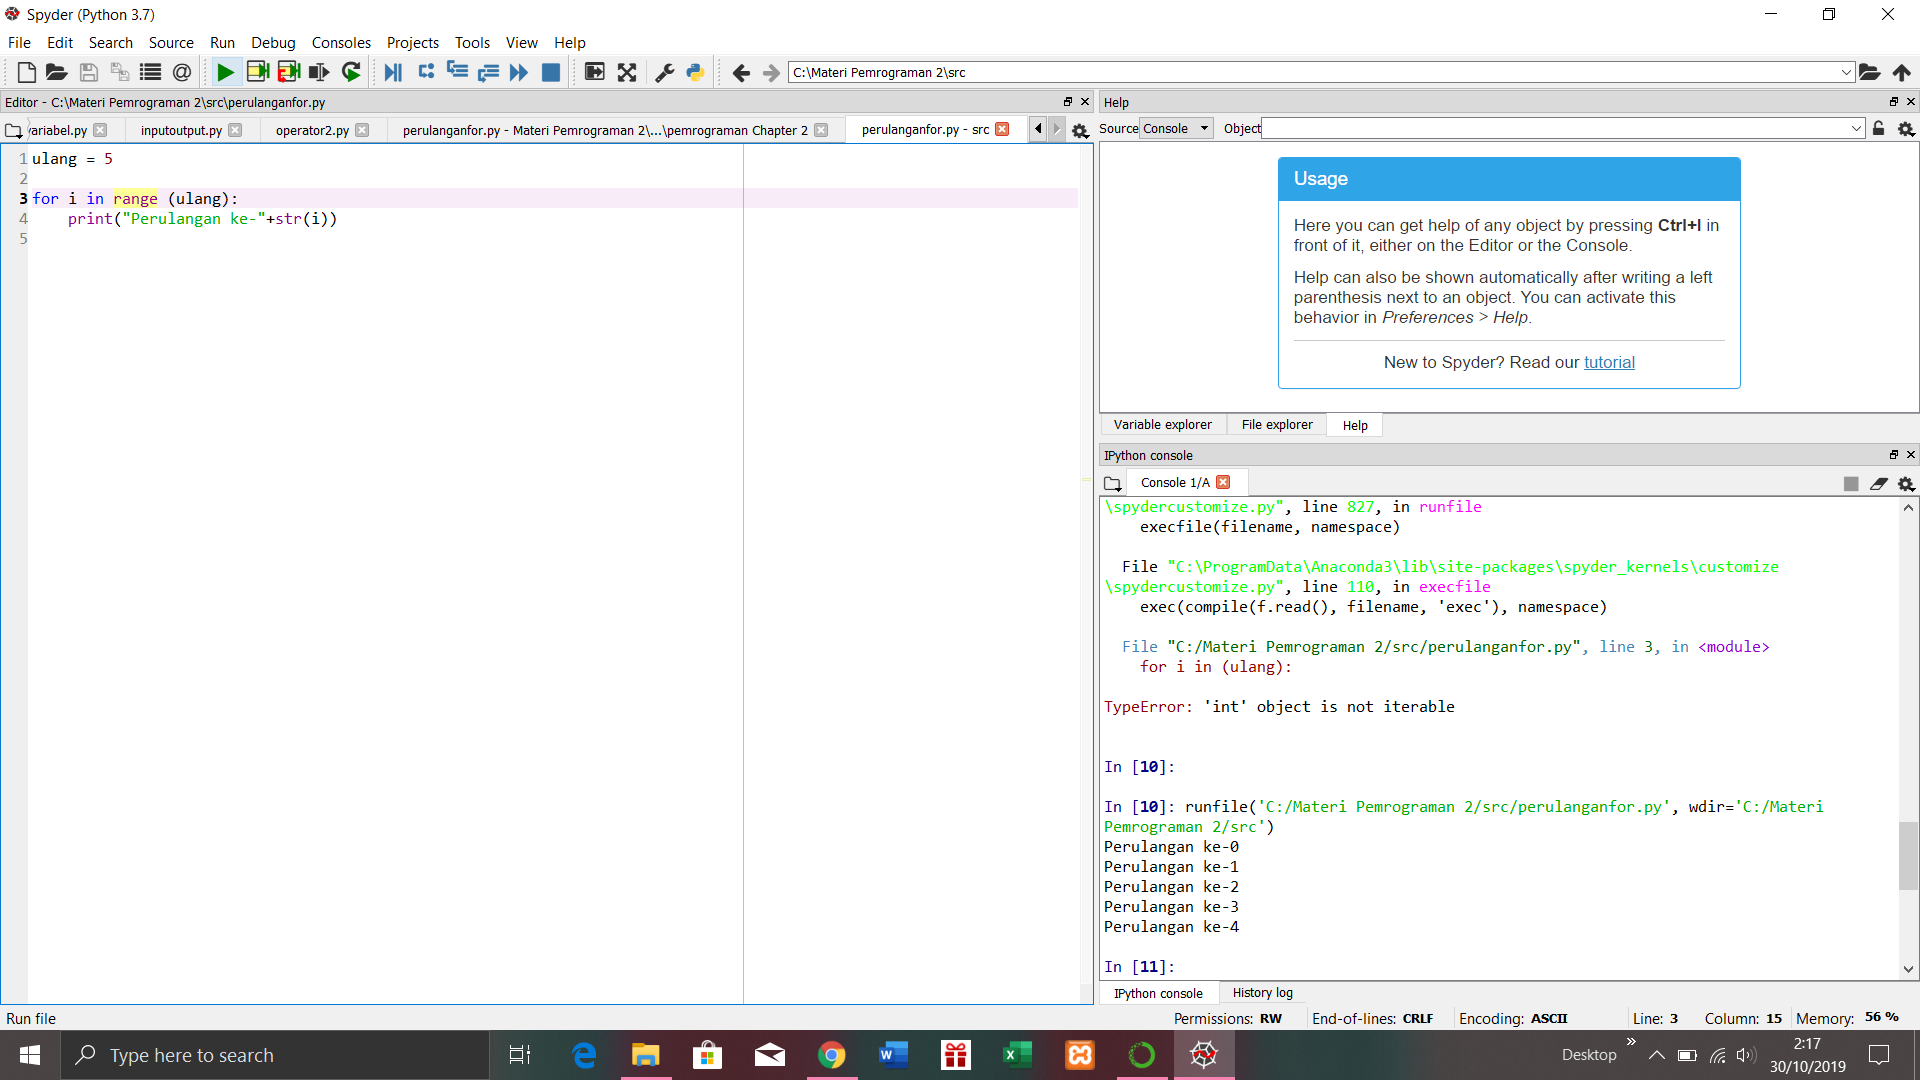
\includegraphics[width=8cm]{figures/perulanganfor.png}}
    \lstinputlisting[language=Python]{figures/src/perulanganfor.py}
    \item Perulangan While
    \par Bila kondisi yang diuji salah, maka loop tidak akan pernah dieksekusi
    \begin{figure}[h]
                 \centerline{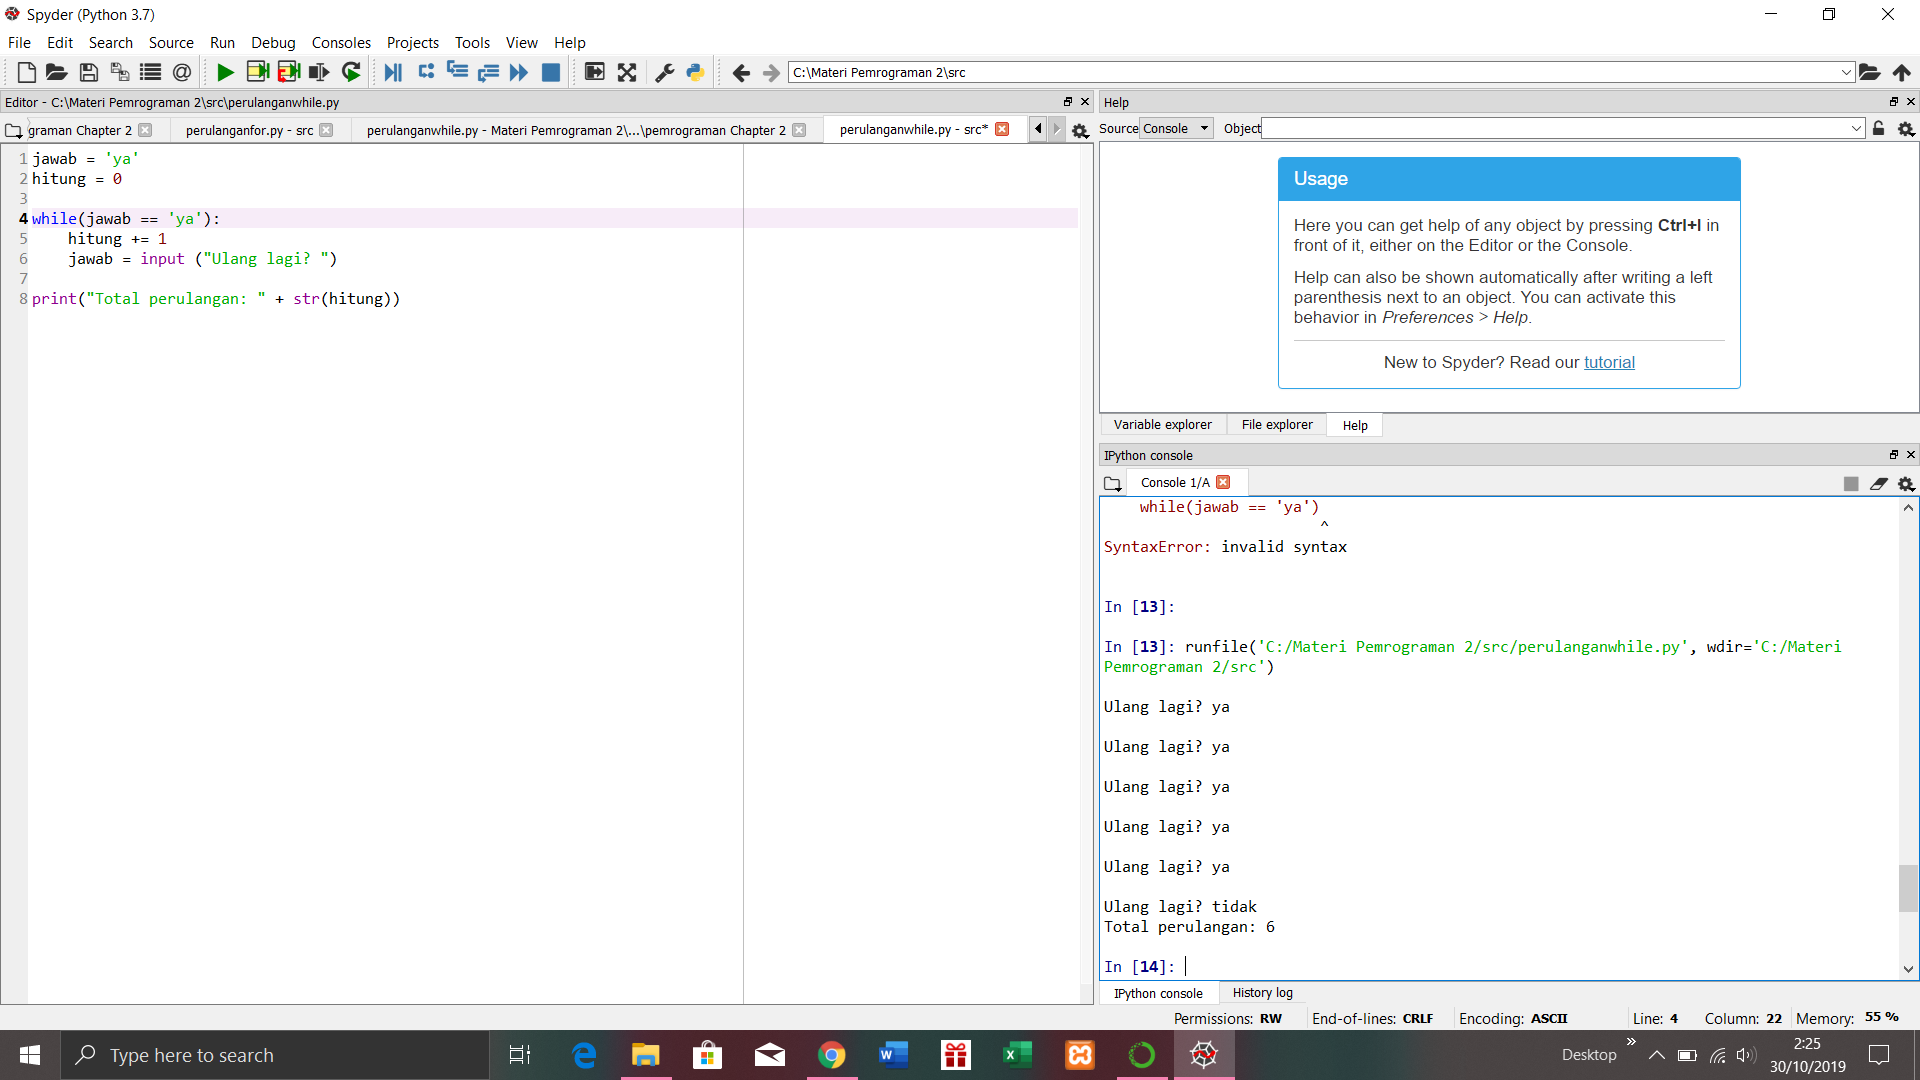
\includegraphics[width=8cm]{figures/perulanganwhile.png}}
        \end{figure}
\lstinputlisting[language=Python]{figures/src/perulanganwhile.py}
\end{enumerate}

\subsection{Cara Menggunakan Syntax Untuk Memilih Kondisi dan Contoh Syntax Kondisi Di Dalam Kondisi}
\paragraph{}
        Python memiliki tiga jenis kondisional yang dapat digunakan untuk membangun suatu alur logika.adalah  if, ifelse, dan ifelifelse. 
\begin{enumerate}
    \item Kondisi If
    \par Jika kondisi utama true, maka perintah akan dijalankan
    \begin{figure}[h]
        \centerline{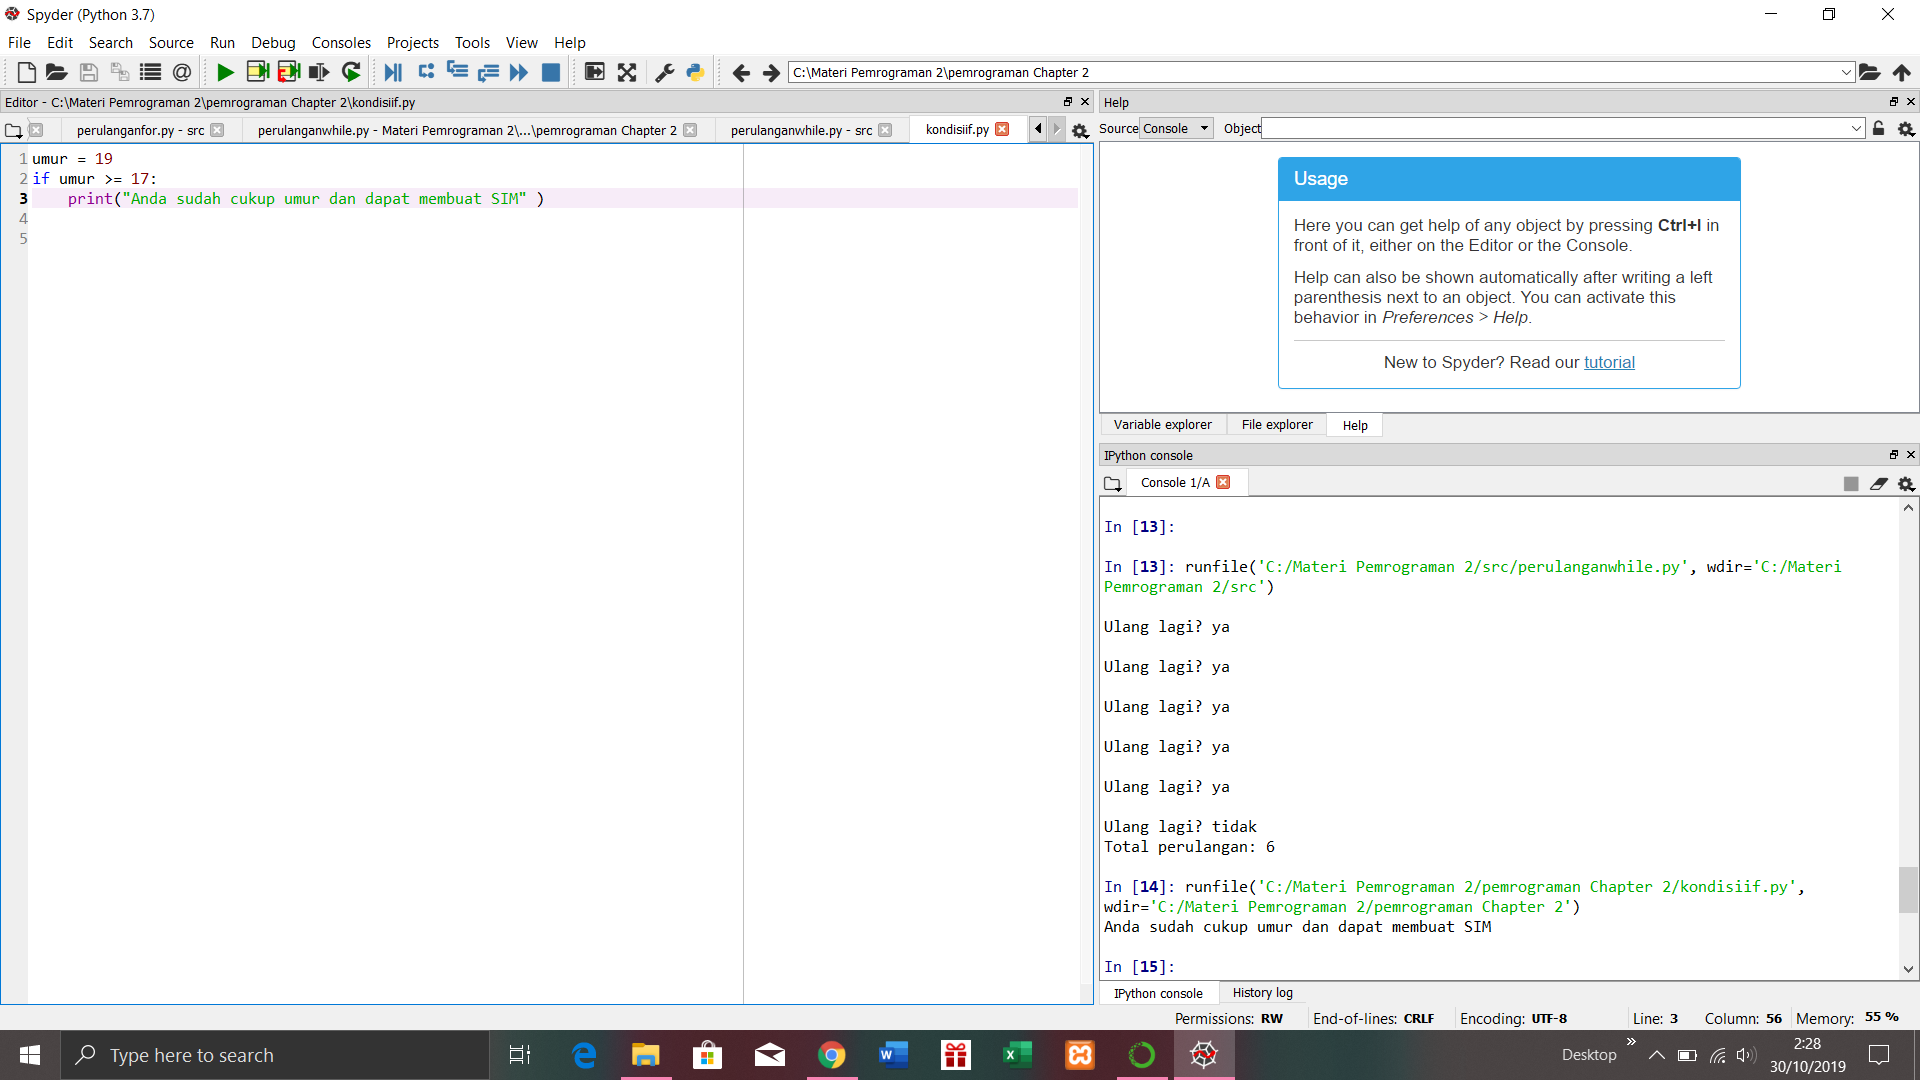
\includegraphics[width=8cm]{figures/kondisiif.png}}
    \end{figure}
    \item Kondisi If Else
    \par Untuk memeriksa kondisi utama, else digunakan untuk menangani kondisi selain kondisi yang telah ditentukan.
    \paragraph{}
    \centerline{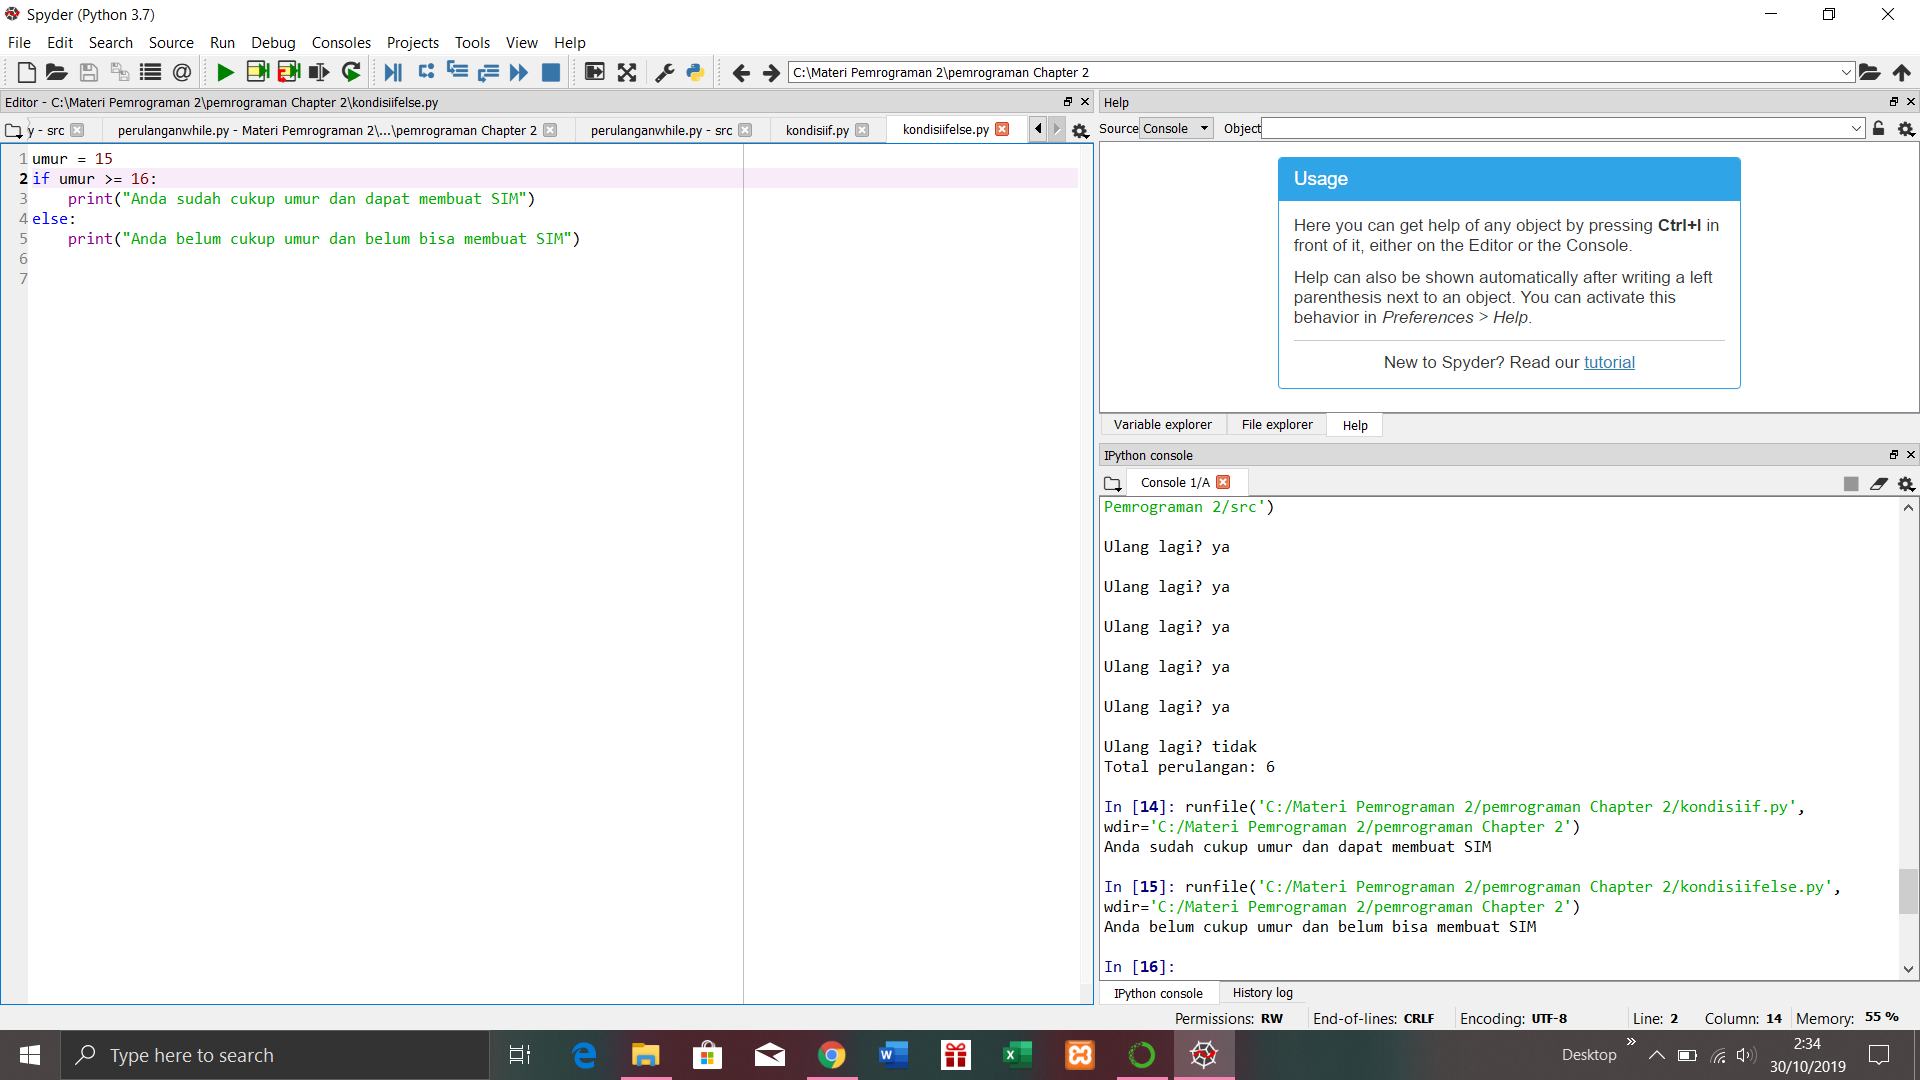
\includegraphics[width=8cm]{figures/kondisiifelse.png}}
    \item Kondisi if elif else
    \par Bila anda akan mendefinisikan cukup banyak kondisi, maka gunakan elif di bawah statement if dan diatas statement else.
  
  \begin{figure}[h]
        \centerline{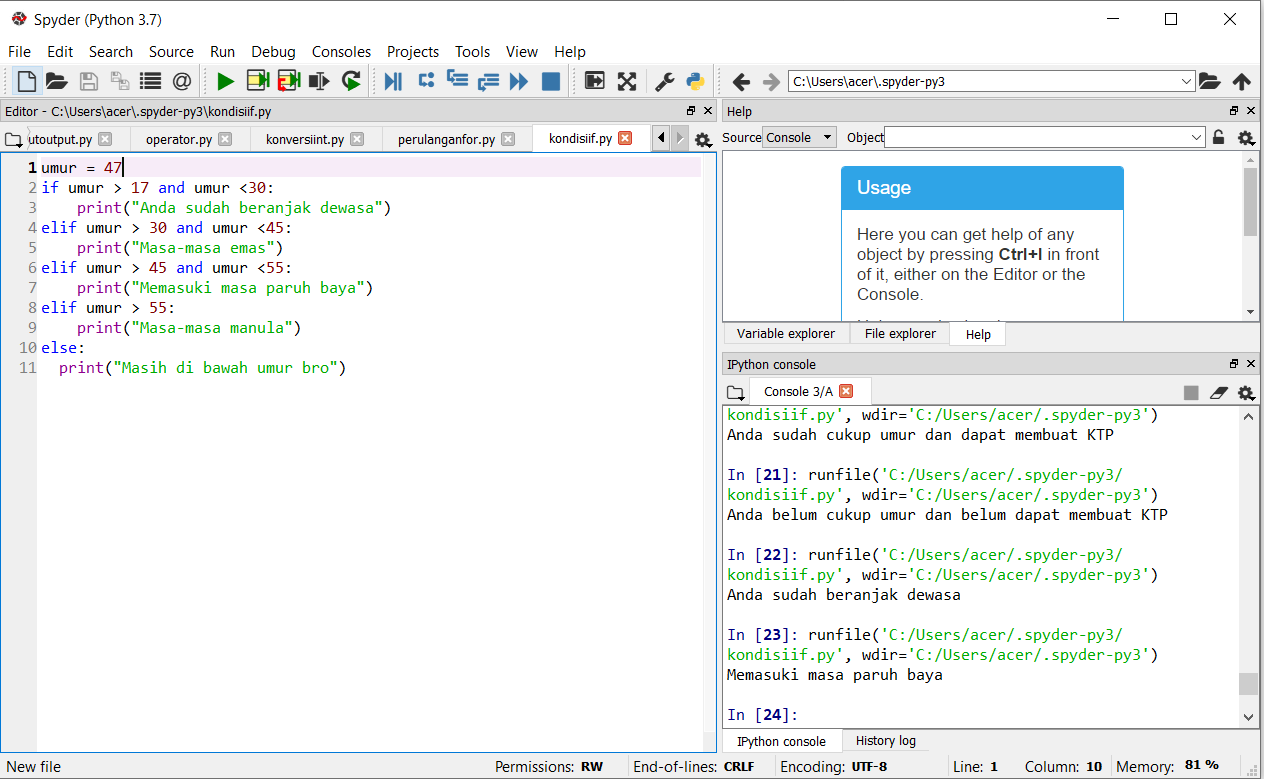
\includegraphics[width=8cm]{figures/kondisiifelifelse.png}}
    \end{figure}
    \item If di dalam if (If bersarang)
    \par Suatu kondisional dapat dsimpan di dalam if lain, berikut adalah contohnya:
    \begin{figure}[h]
        \centerline{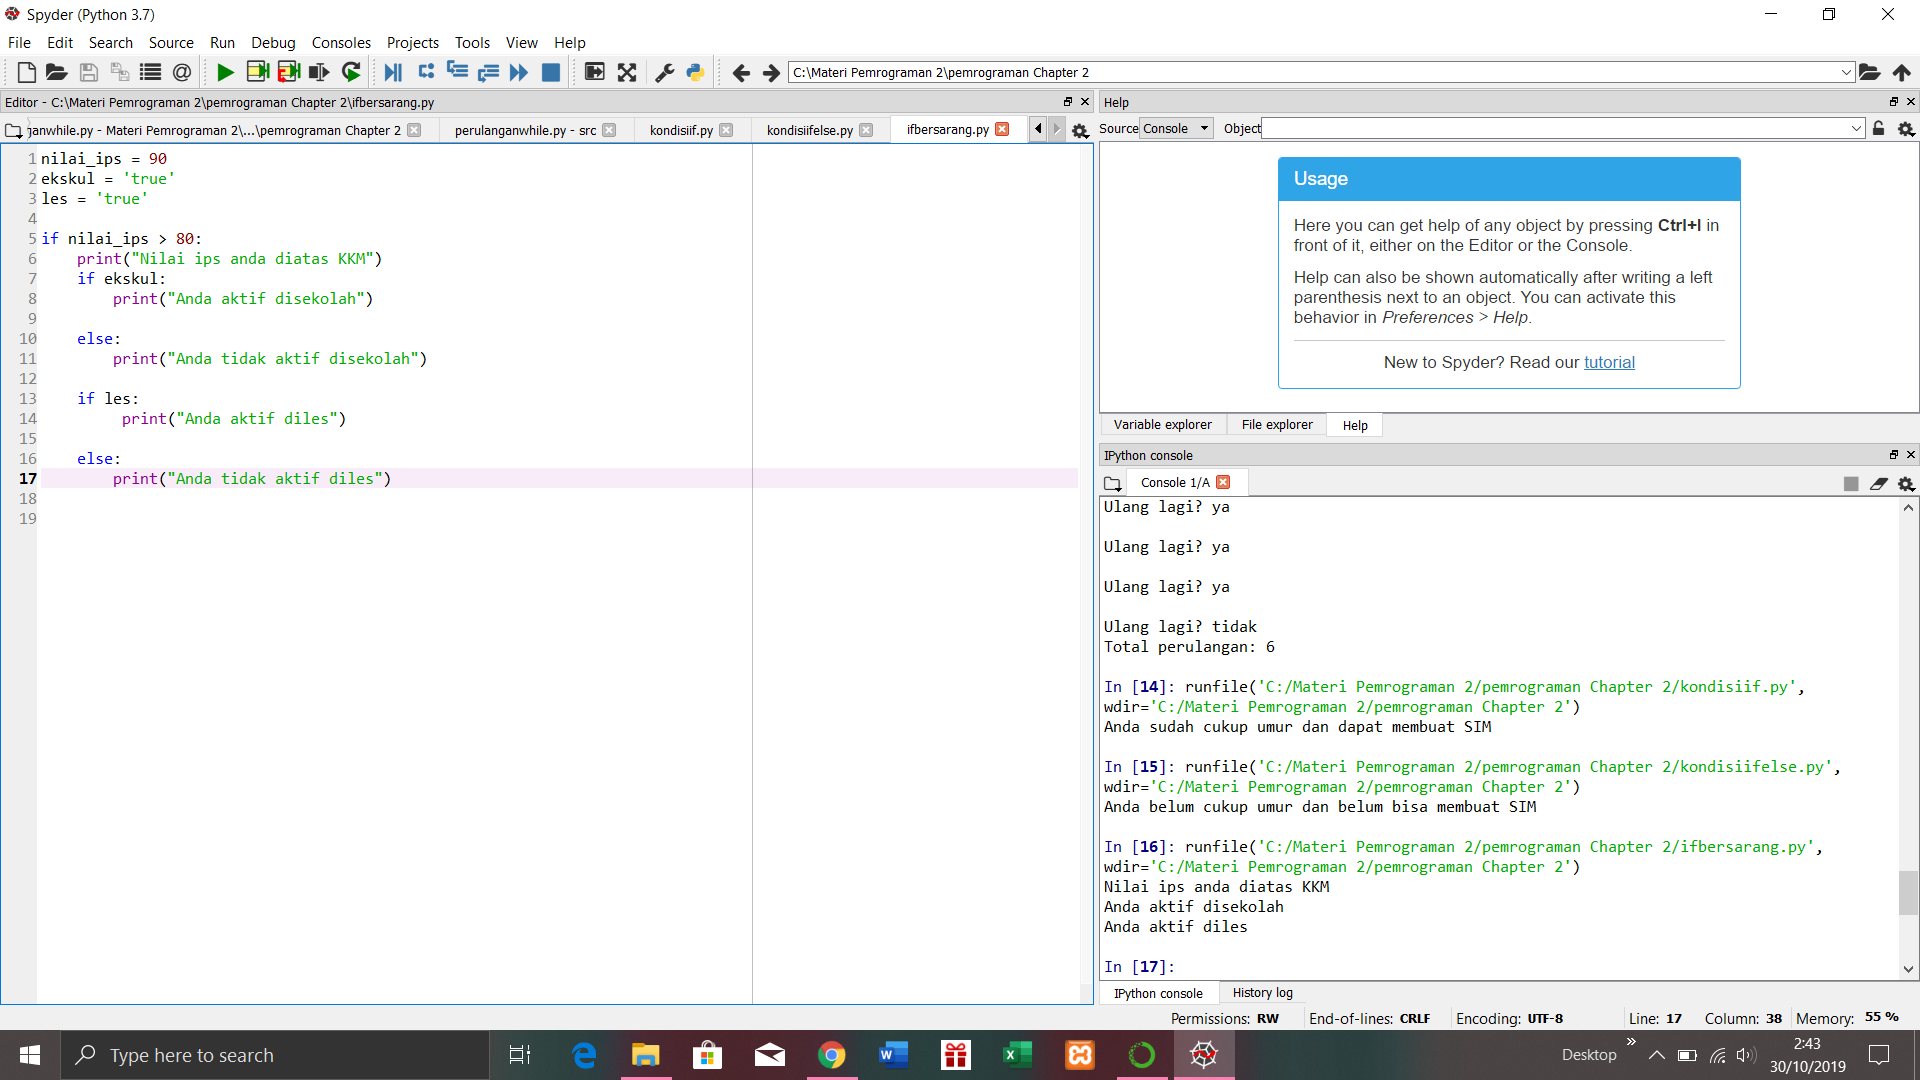
\includegraphics[width=8cm]{figures/ifbersarang.png}}
    \end{figure}
\end{enumerate}

\subsection{Jenis error yang sering ditemui di Python dalam mengerjakan Syntax di atas}
\paragraph{}
        Biasanya error terjadi dikarenakan ada kesalahan dalam pengetikan syntax, contohnya sebagai berikut:
        \begin{figure}[h]
        \centerline{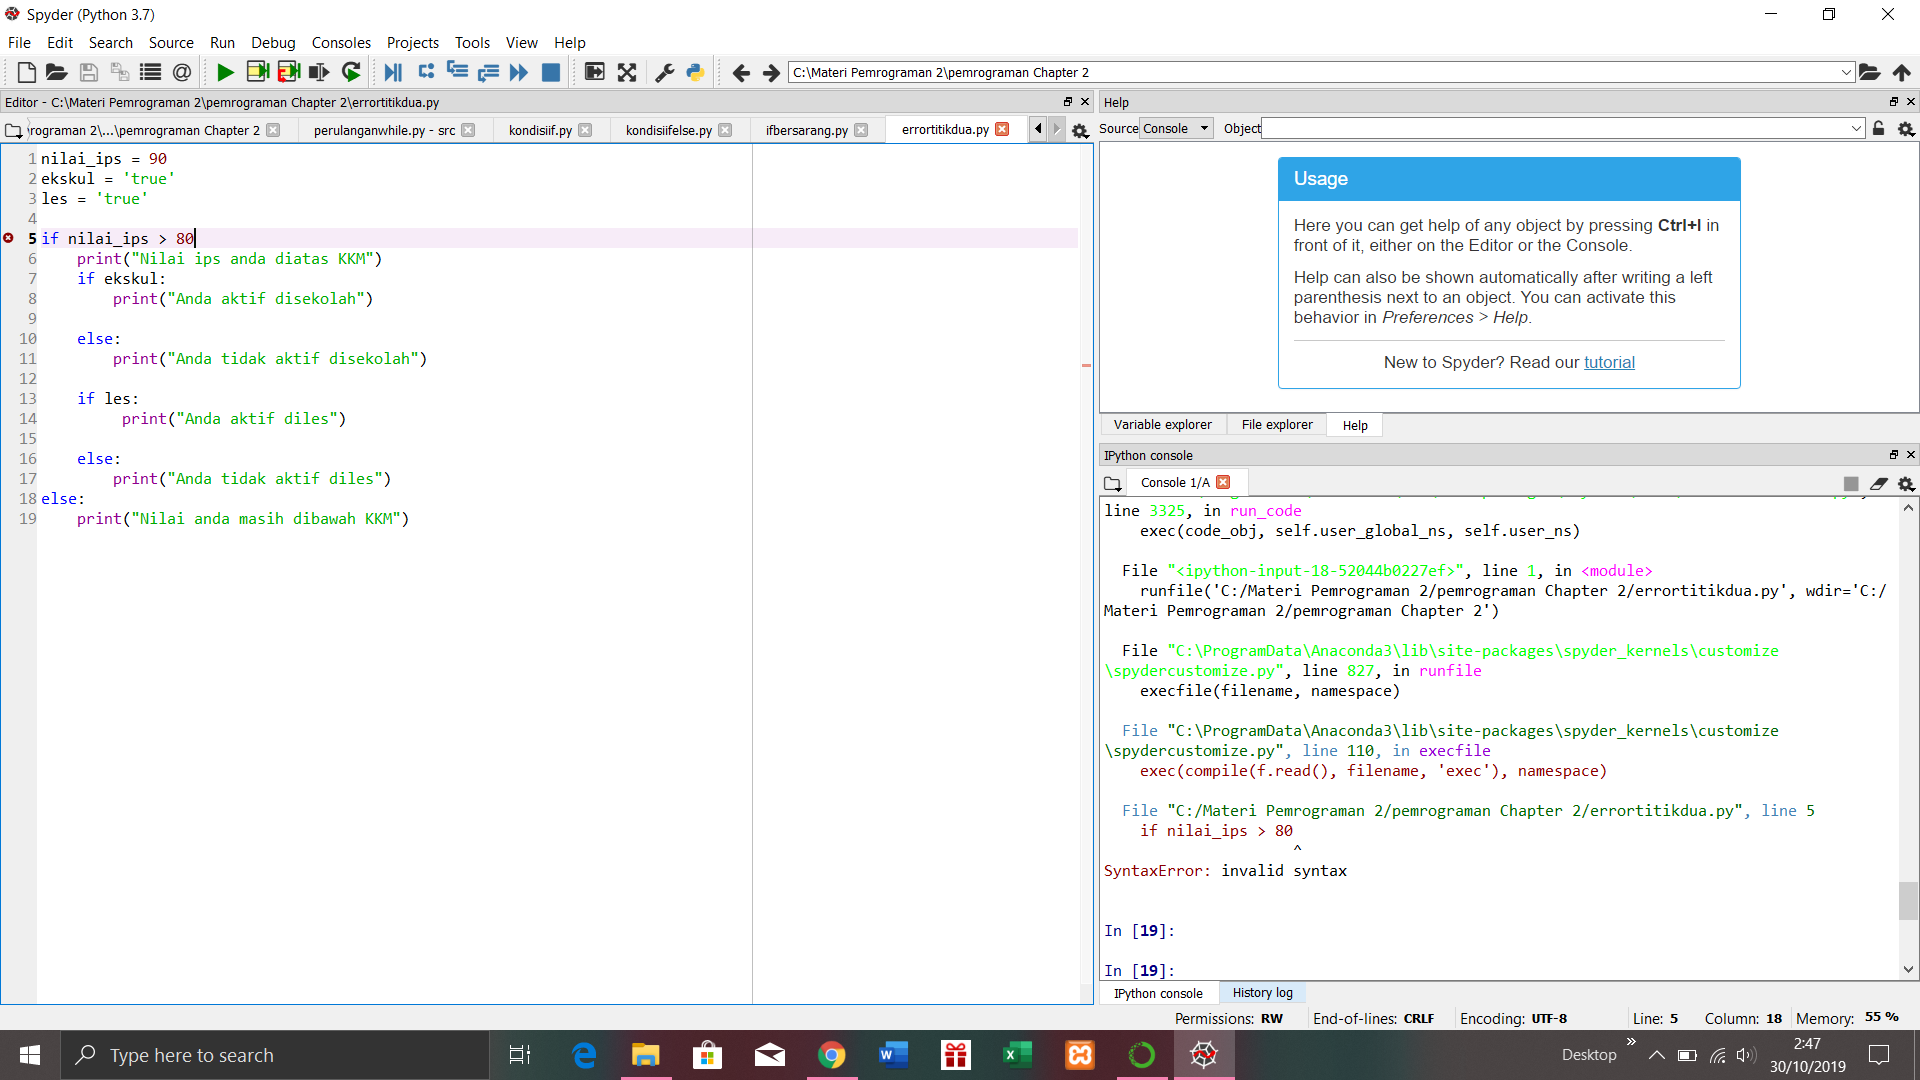
\includegraphics[width=8cm]{figures/errortitikdua.png}}
        \end{figure}
        \par Gambar di atas merupakan contoh dari kesalahan syntax titik dua pada line 5.
        \begin{figure}[h]
        \centerline{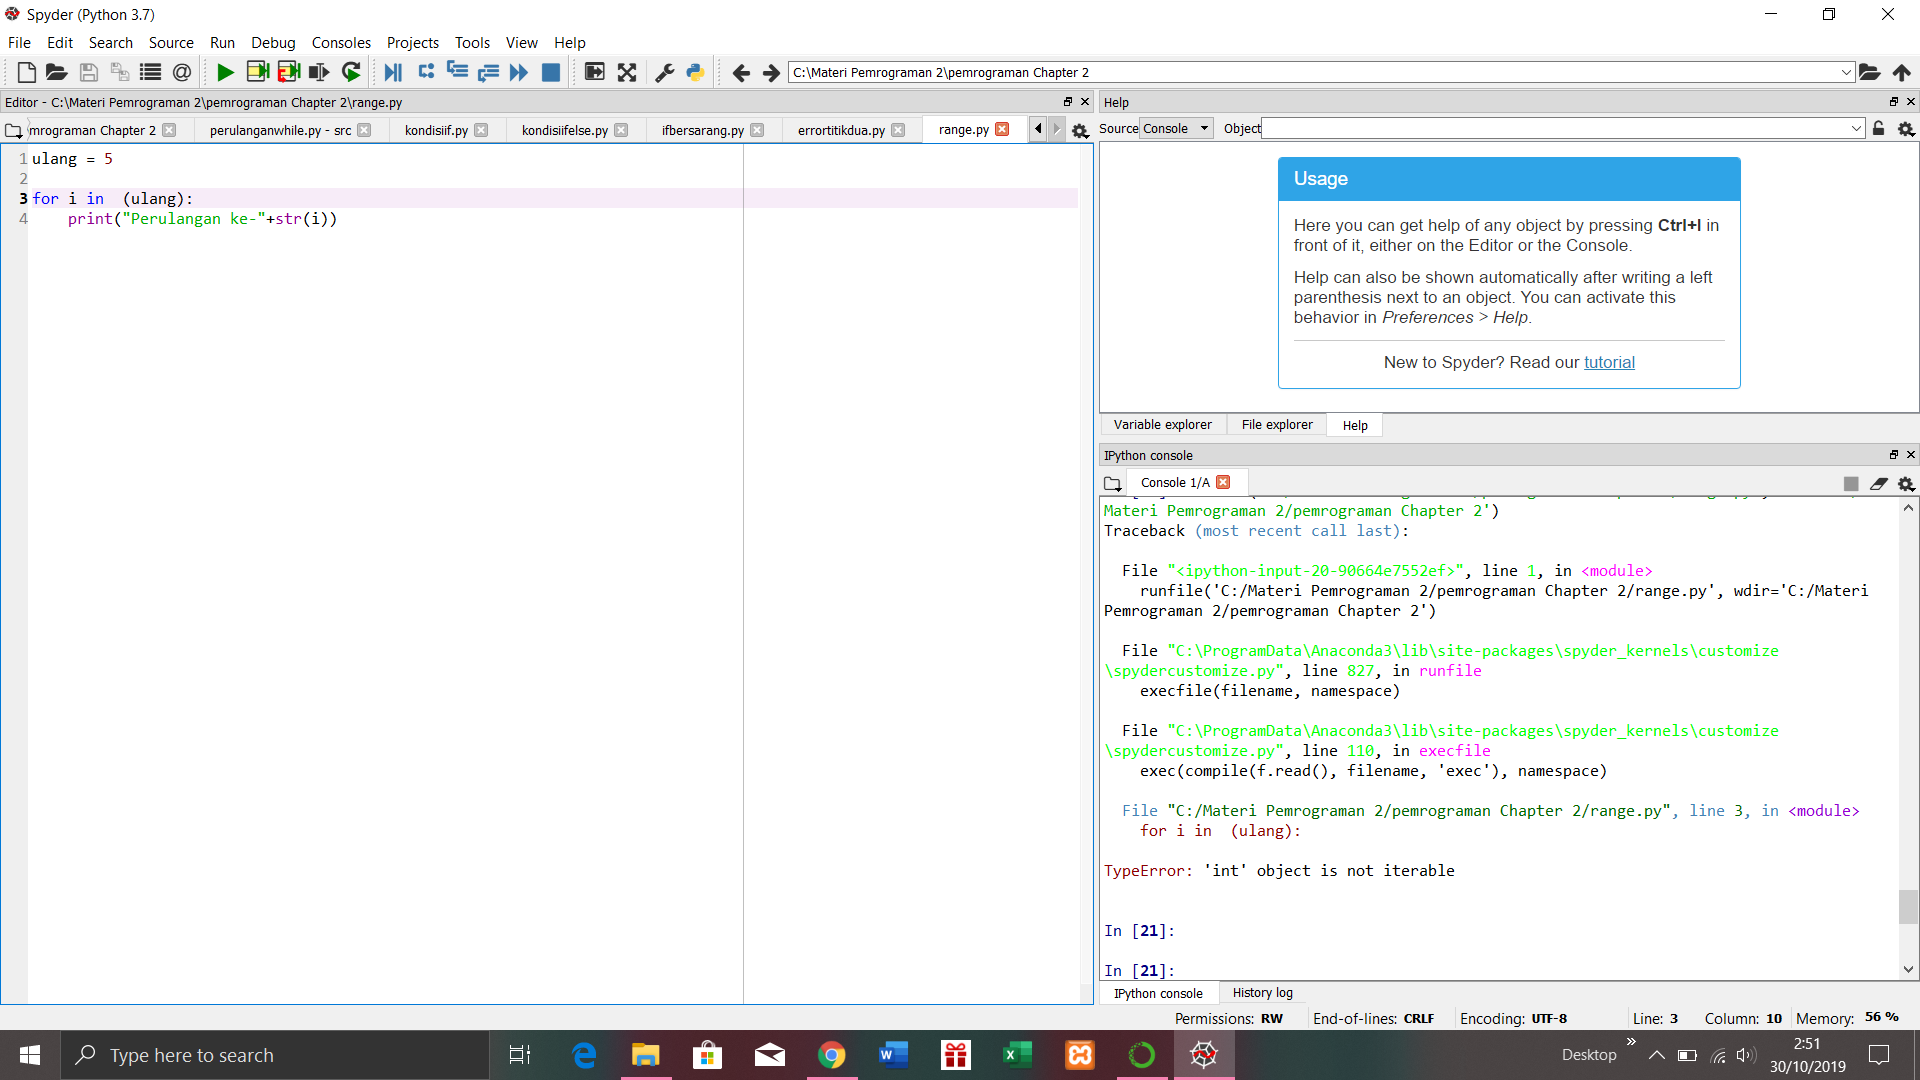
\includegraphics[width=8cm]{figures/range.png}}
        \end{figure}
        \par Gambar di atas merupakan contoh dari kesalahan syntax range, jika nilai bertipe data integer maka harus menggunakan range setelah in.

\subsection{Cara Memakai Try Except}
\paragraph{}
        Try except biasa digunakan untuk menangani error saat penggunaan IO, database, atau pengaksesan indeks suatu list atau dictionary, dll.
       \paragraph{}
        \centerline{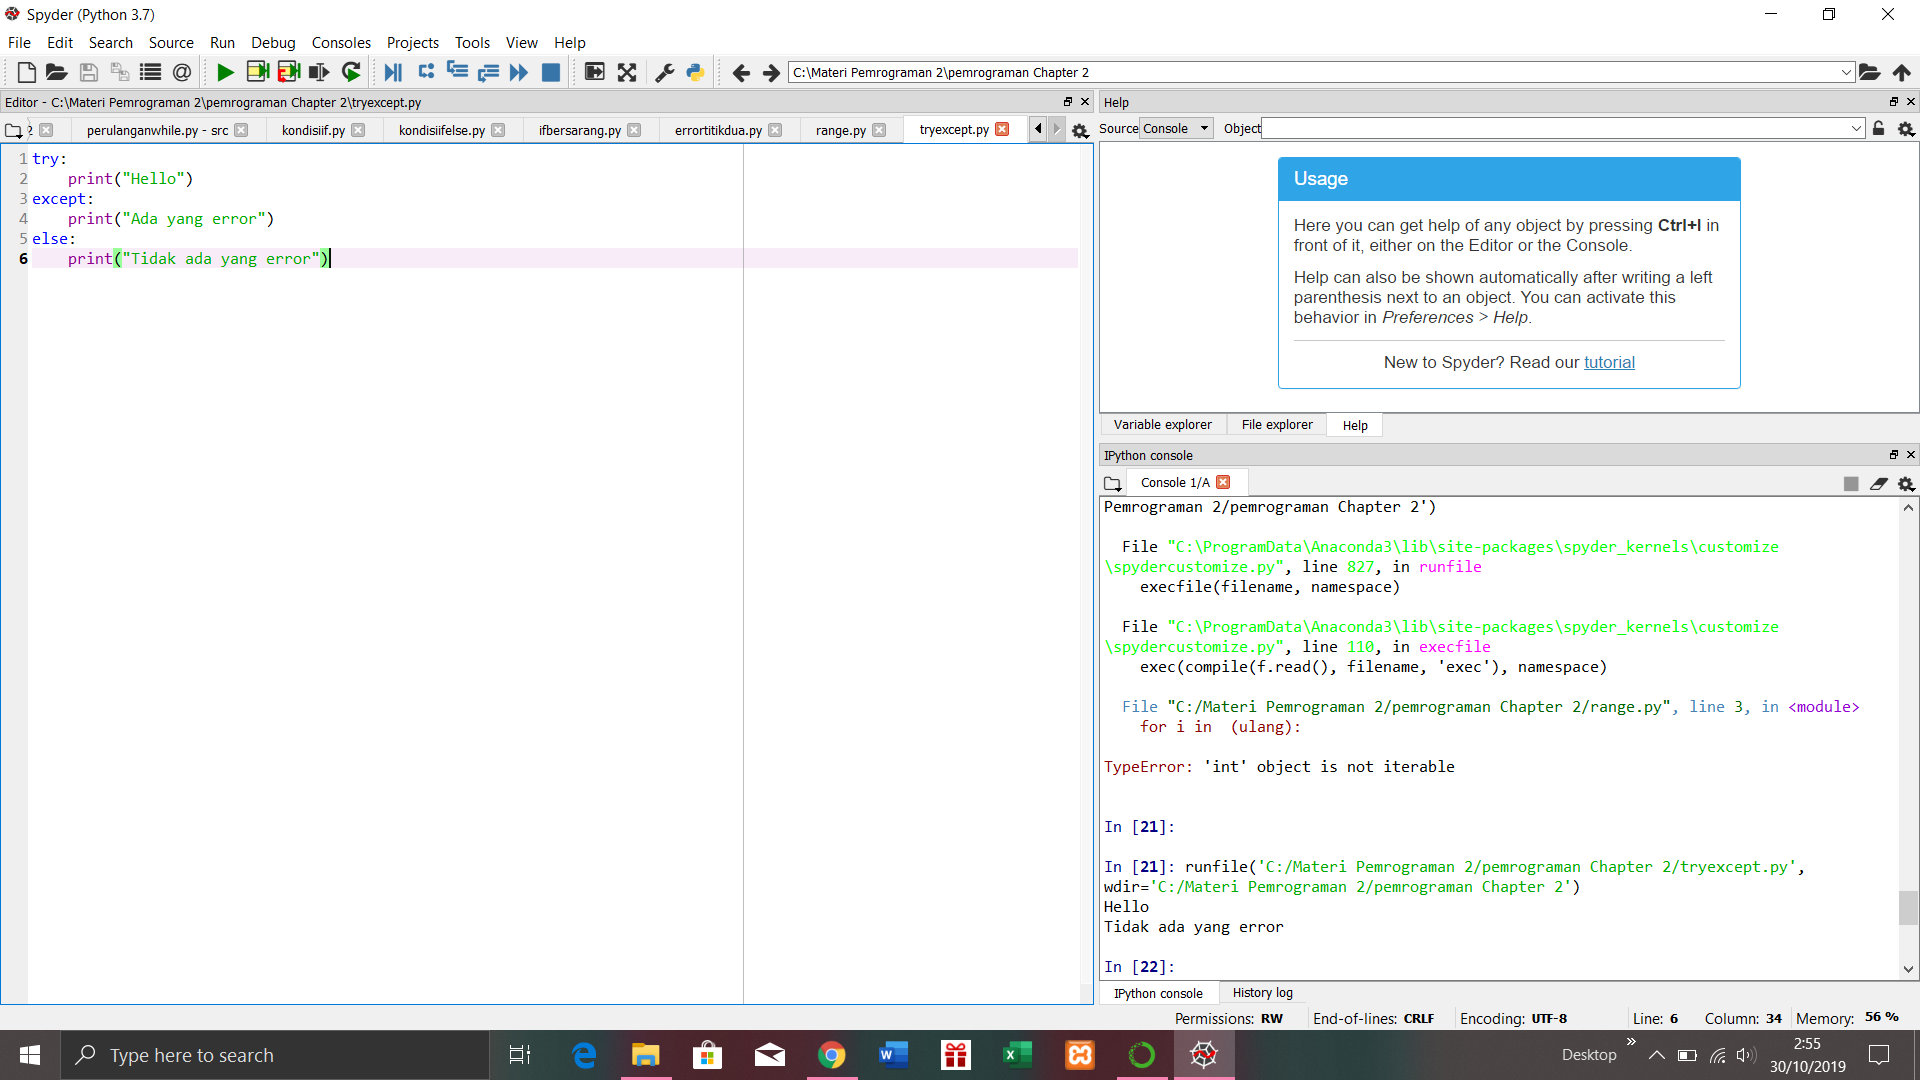
\includegraphics[width=8cm]{figures/tryexcept.png}}

\section{Ketrampilan Pemrograman}
\begin{enumerate}
\item
Luaran huruf yang dirangkai dari tanda bintang, pagar atau plus dari NPM kita.
Tanda bintang untuk NPM mod 3=0, tanda pagar untuk NPM mod 3 =1, tanda plus untuk NPM mod3=2.
Output:
\begin{figure}[h]
\centerline{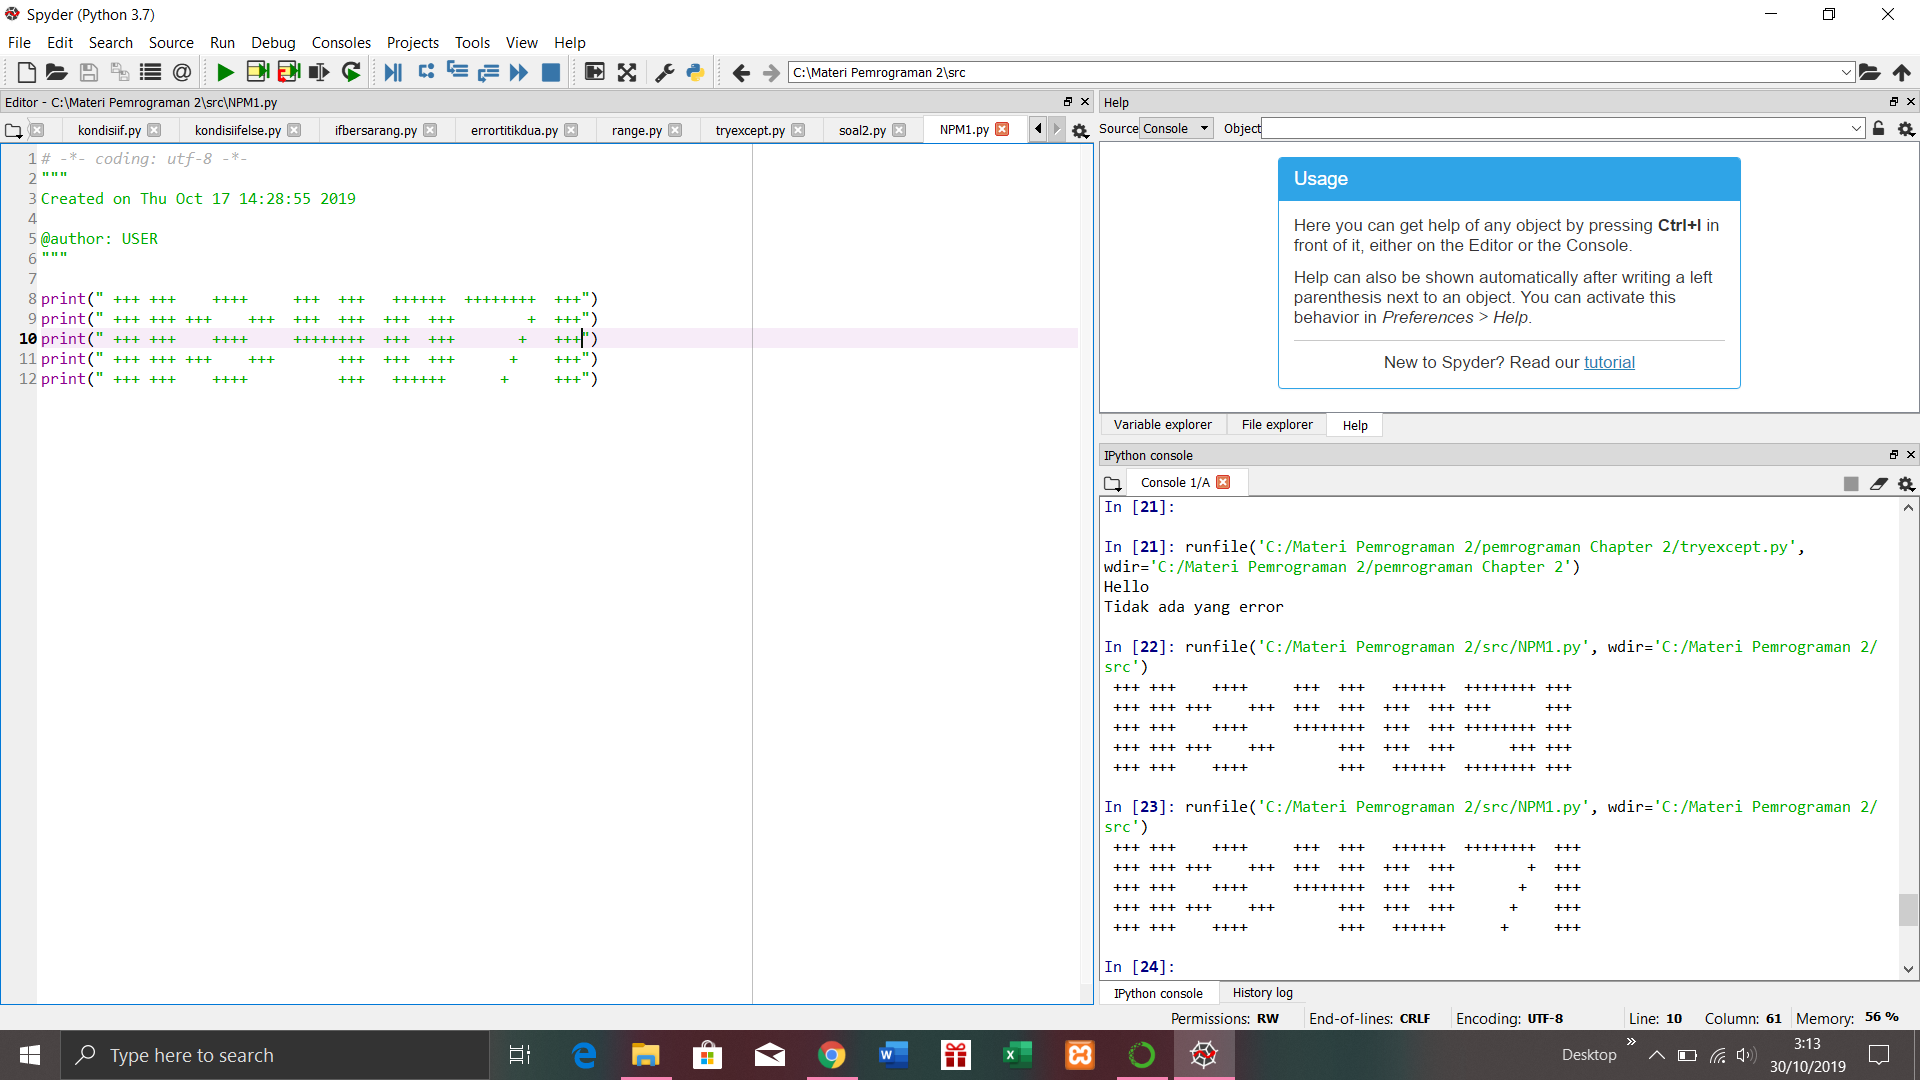
\includegraphics[width=8cm]{figures/NPM11.png}}
\end{figure}
\lstinputlisting[language=Python]{figures/src/NPM1.py}

\item
Program hello word dengan input NPM yang disimpan dalam sebuah variabel string bernama \textbf{NPM} dan output sebanyak dua dijit belakang NPM, 
contoh NPM : 1184071 maka akan ada output sebanyak 87 dengan tulisan `Hallo, 1181071 apa kabar?'
\paragraph{}
\centerline{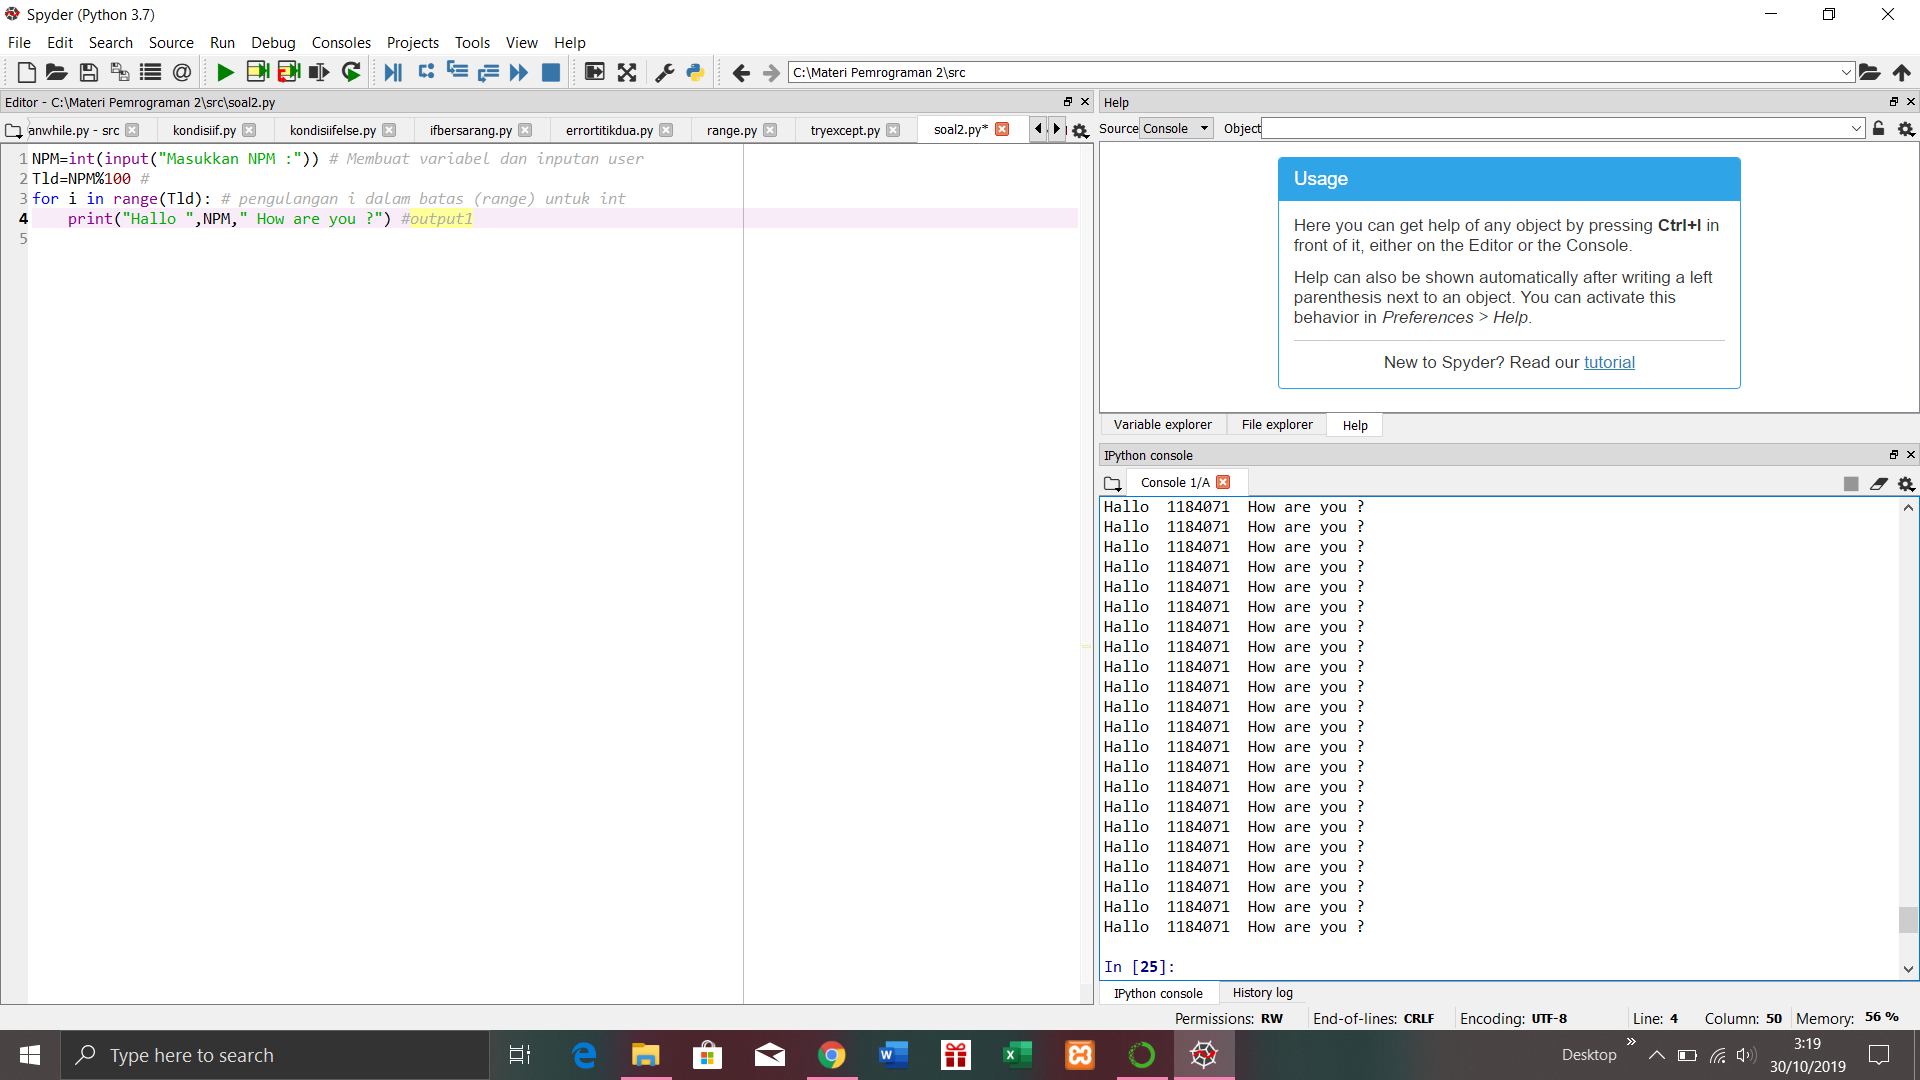
\includegraphics[width=8cm]{figures/soal2.png}}
\lstinputlisting[language=Python]{figures/src/soal2.py}

\item
Program hello word dengan input nama yang disimpan dalam sebuah variabel string bernama \textbf{NPM} dan beri luaran output berupa tiga karakter belakang dari NPM sebanyak penjumlahan tiga dijit tersebut.
\begin{figure}[h]
\centerline{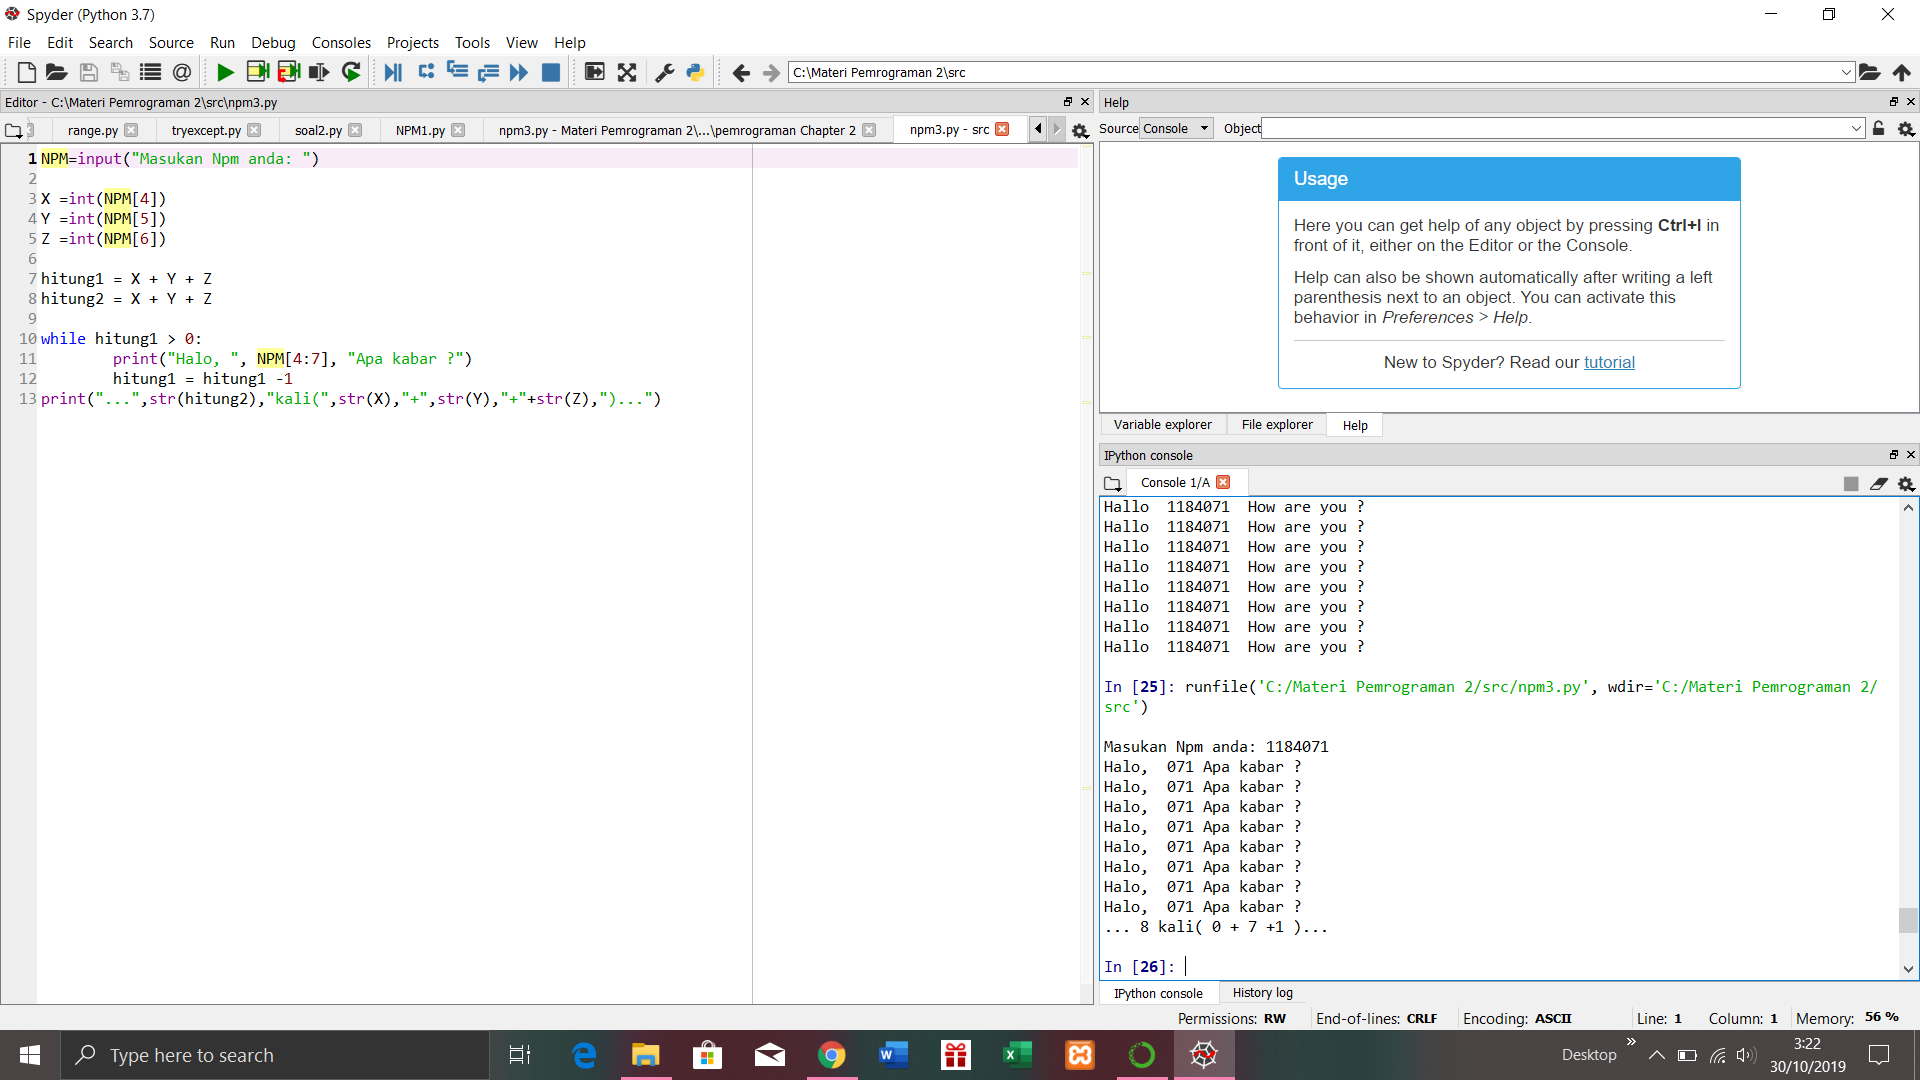
\includegraphics[width=8cm]{figures/npm3.png}}
\end{figure}
\lstinputlisting[language=Python]{figures/src/npm3.py}

\item
Program hello word dengan input nama yang disimpan dalam sebuah variabel string bernama \textbf{NPM} dan beri luaran output berupa digit ketiga dari belakang dari variabel NPM.
\begin{figure}[h]
\centerline{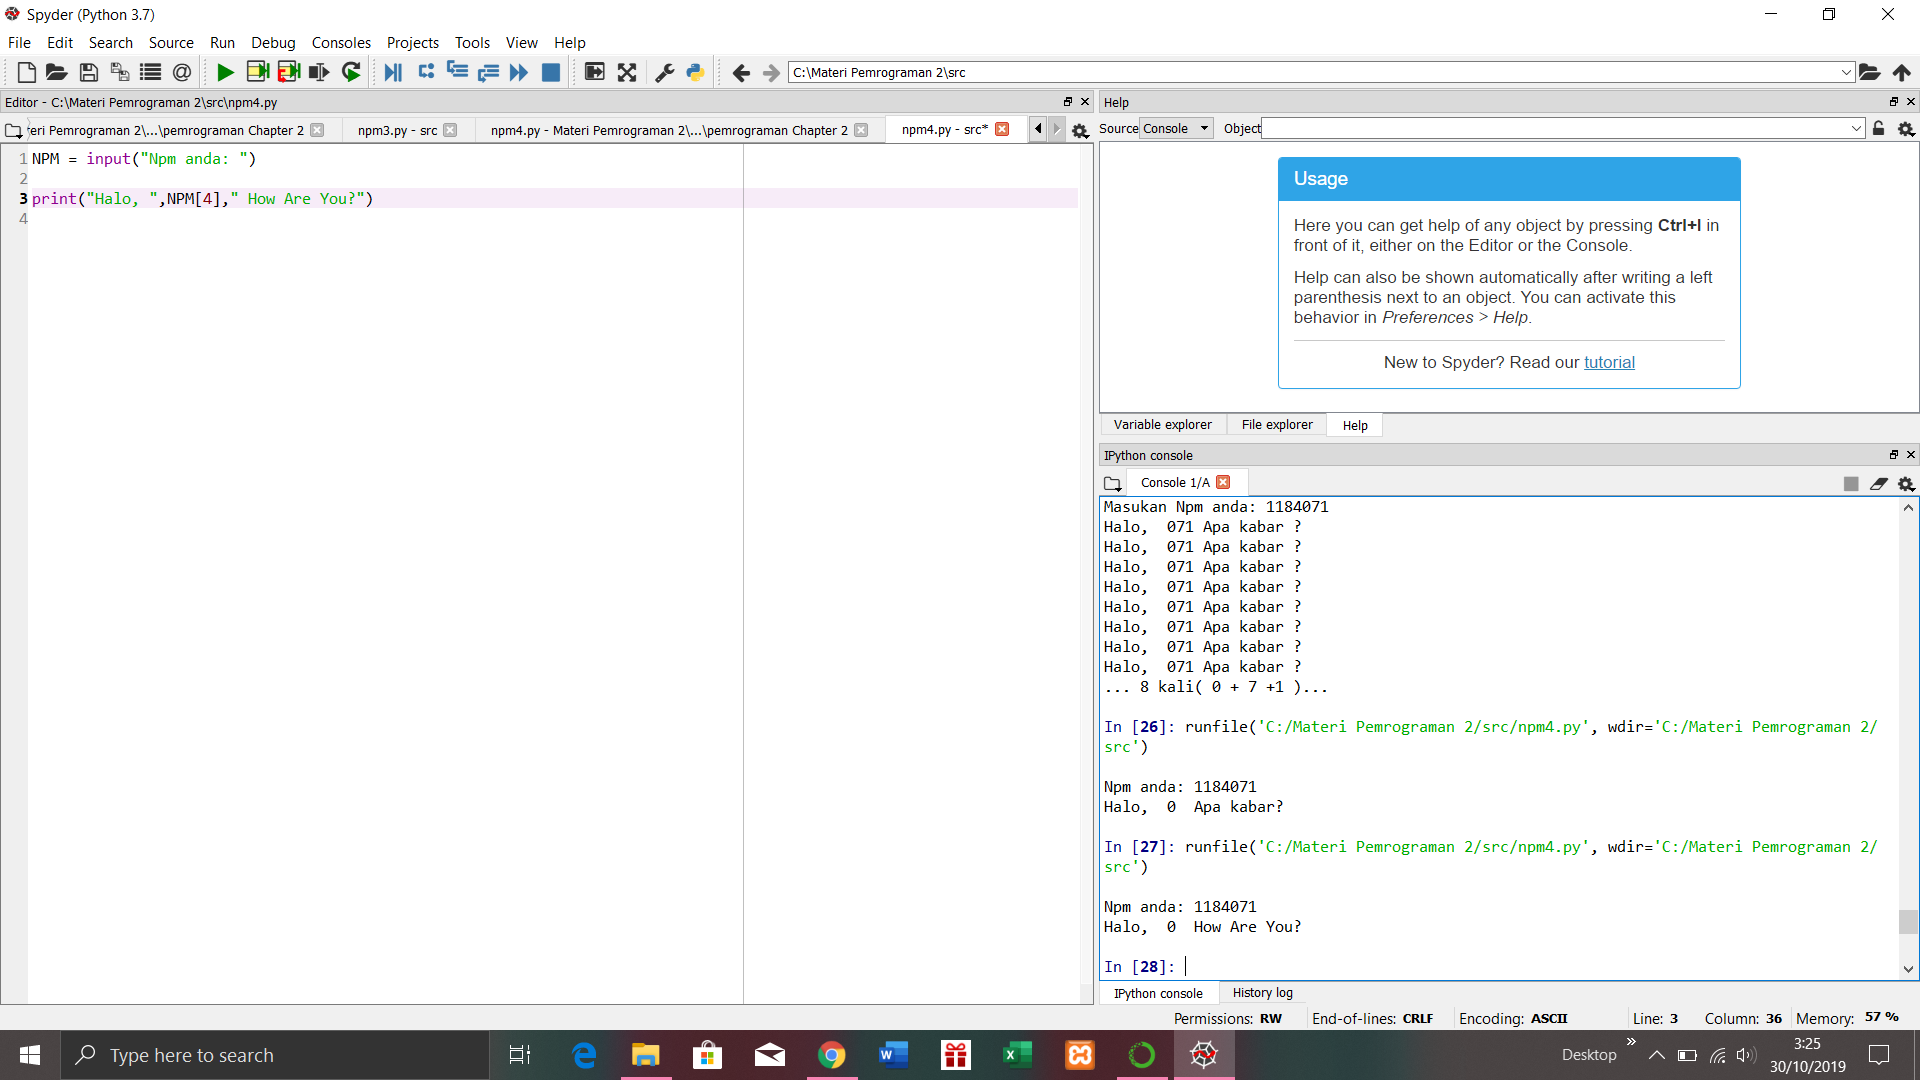
\includegraphics[width=8cm]{figures/npm4.png}}
\end{figure}
\lstinputlisting[language=Python]{figures/src/npm4.py}

\item
\label{digitvar}
(untuk soal no \ref{digitvar} dan selanjutnya wajib menggunakan perulangan dan kondisi) buat program dengan mengisi variabel alfabet dengan nomor npm satu persatu berurut.
\paragraph{}
\centerline{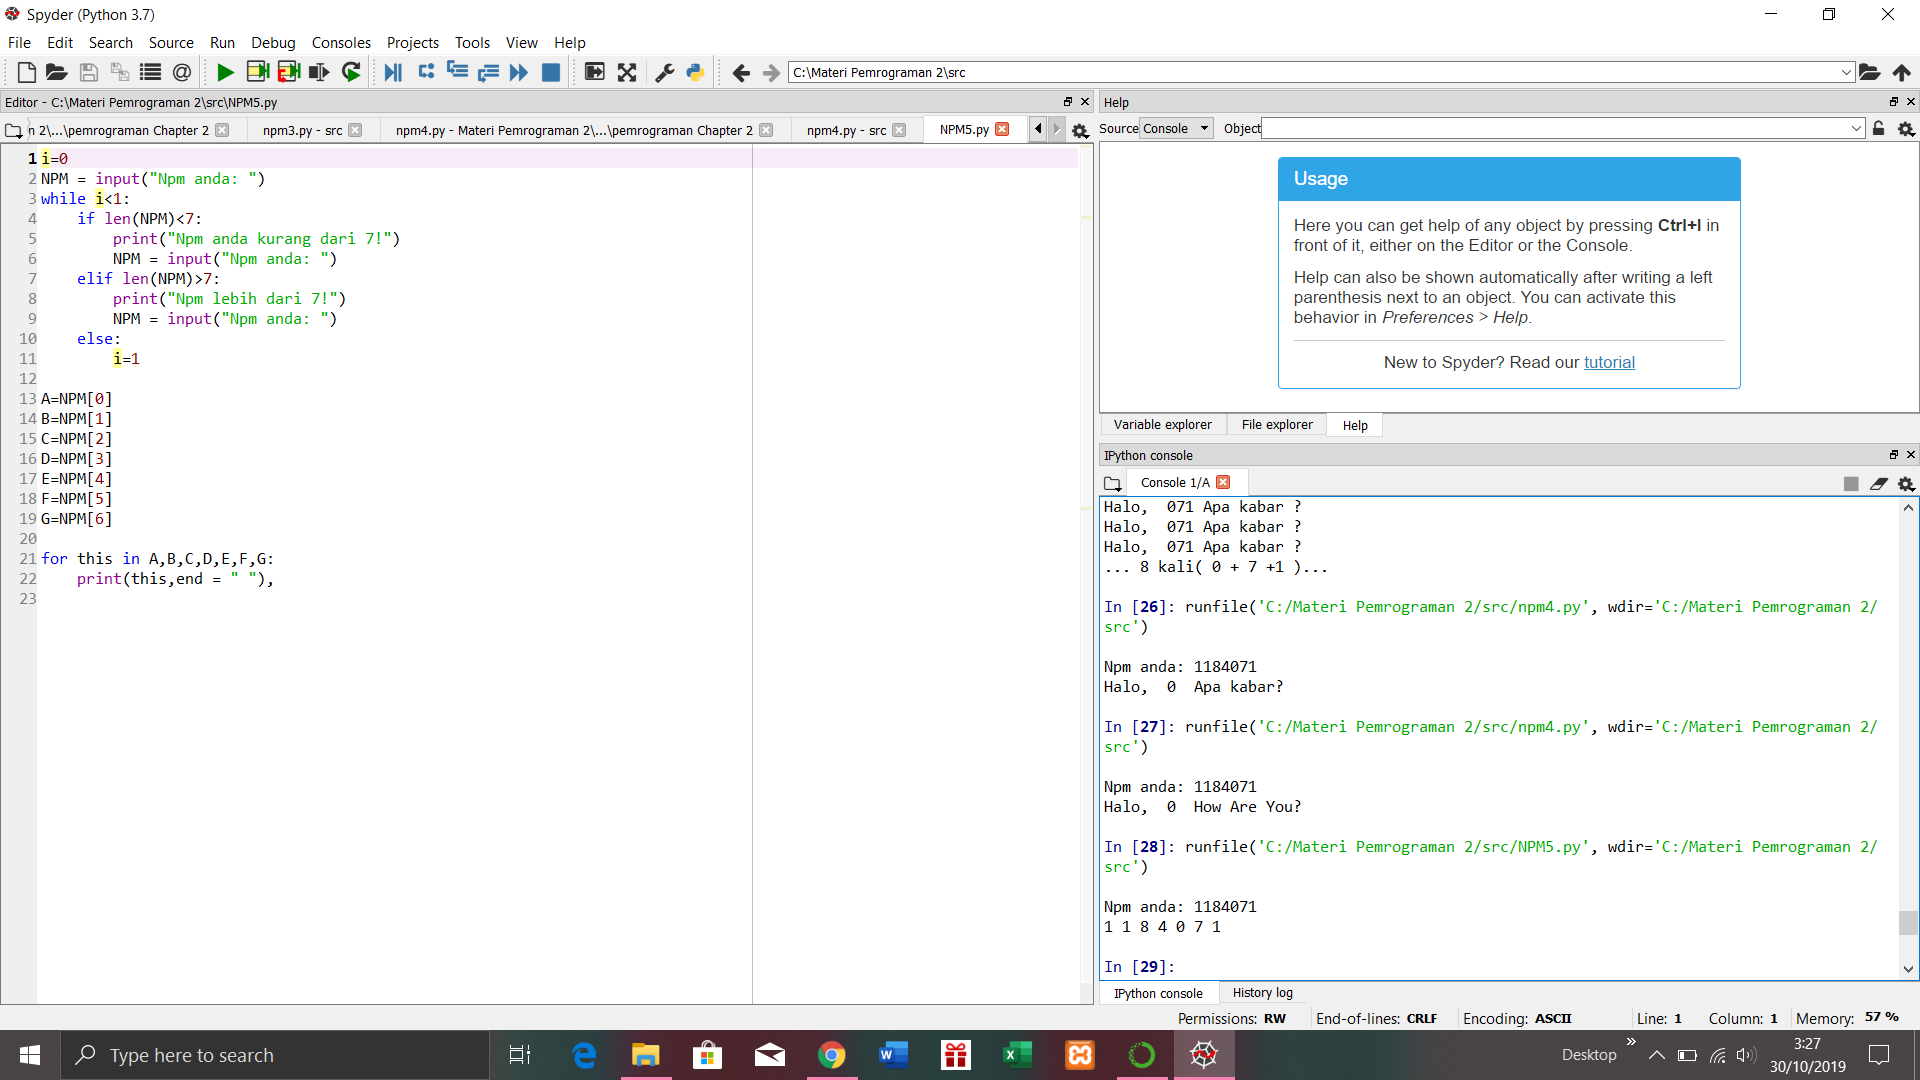
\includegraphics[width=8cm]{figures/npm5.png}}
\lstinputlisting[language=Python]{figures/src/npm5.py}

\item
Dari soal no \ref{digitvar}, Lakukan penjumlahan dari seluruh variabel tersebut
\begin{figure}[h]
\centerline{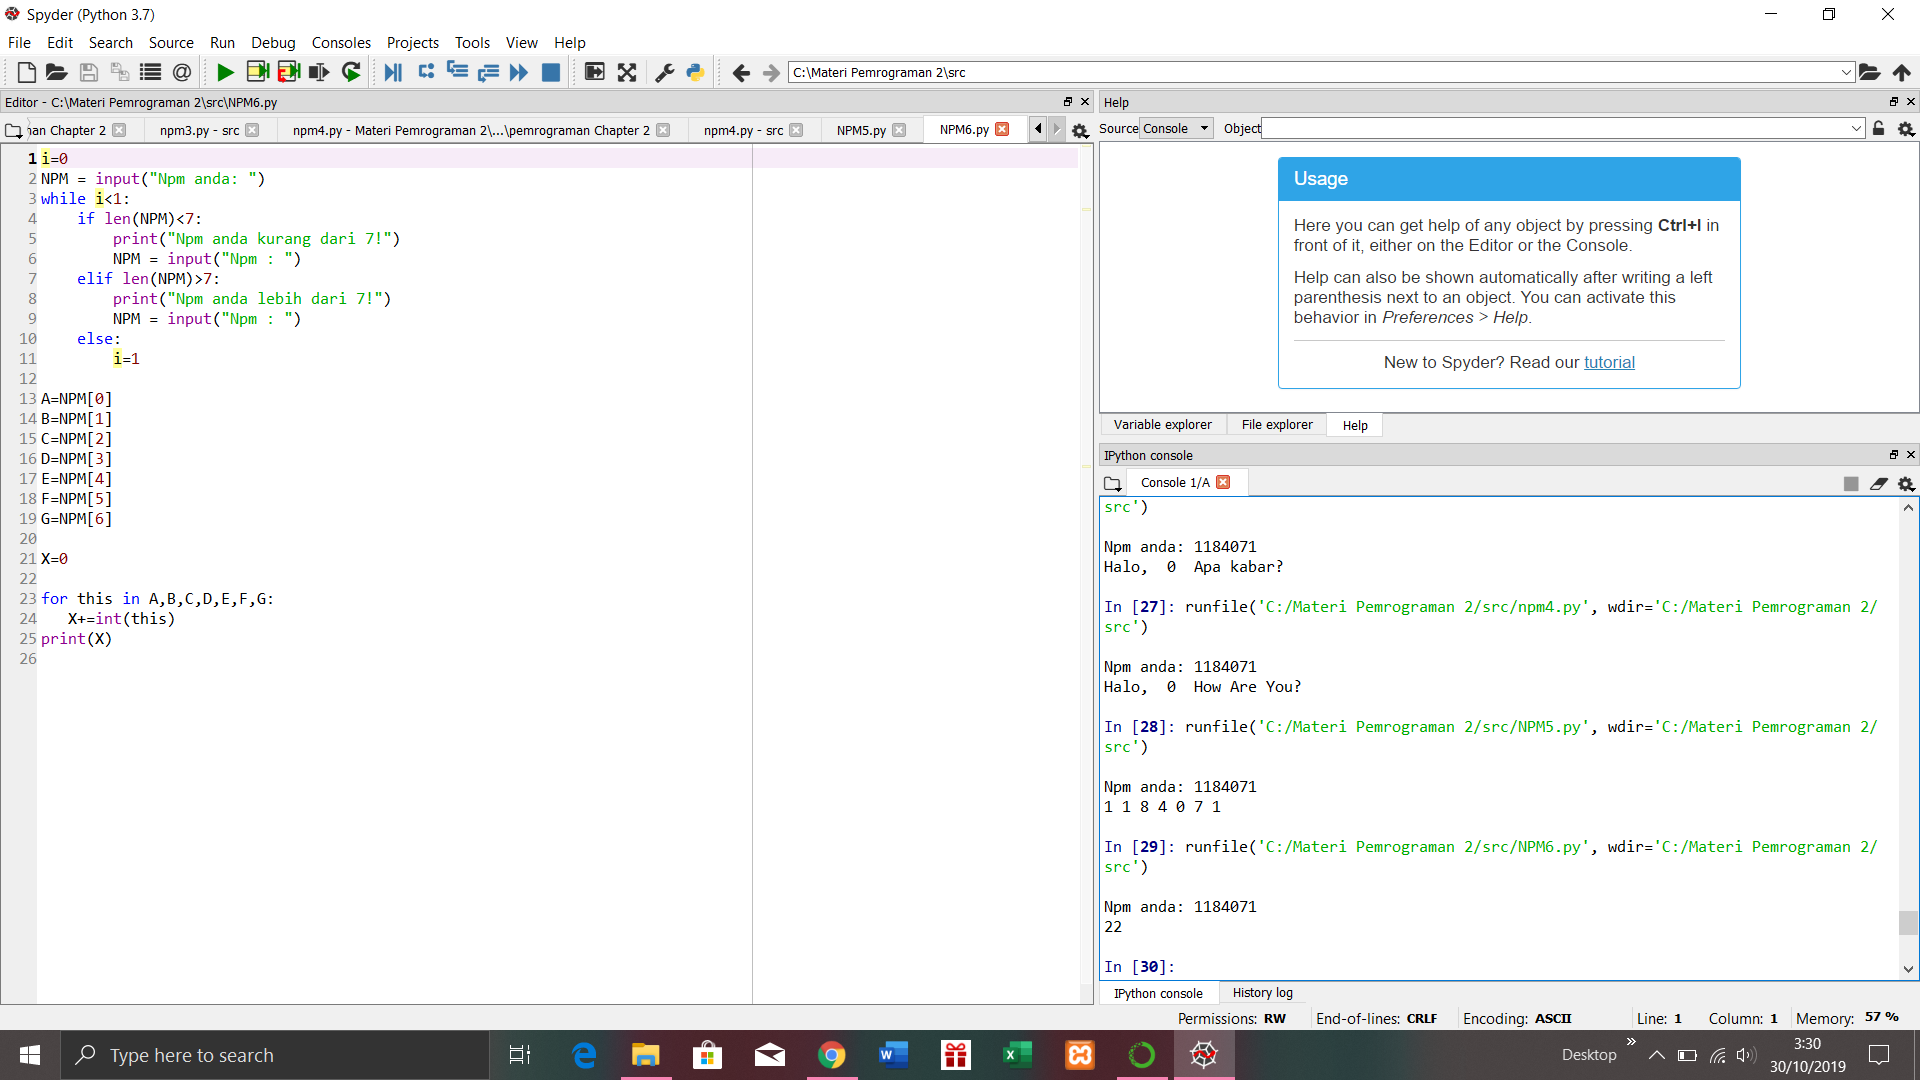
\includegraphics[width=8cm]{figures/npm6.png}}
\end{figure}
\lstinputlisting[language=Python]{figures/src/npm6.py}

\item 
Dari soal no \ref{digitvar}, Lakukan perkalian dari seluruh variabel tersebut
\begin{figure}[h]
\centerline{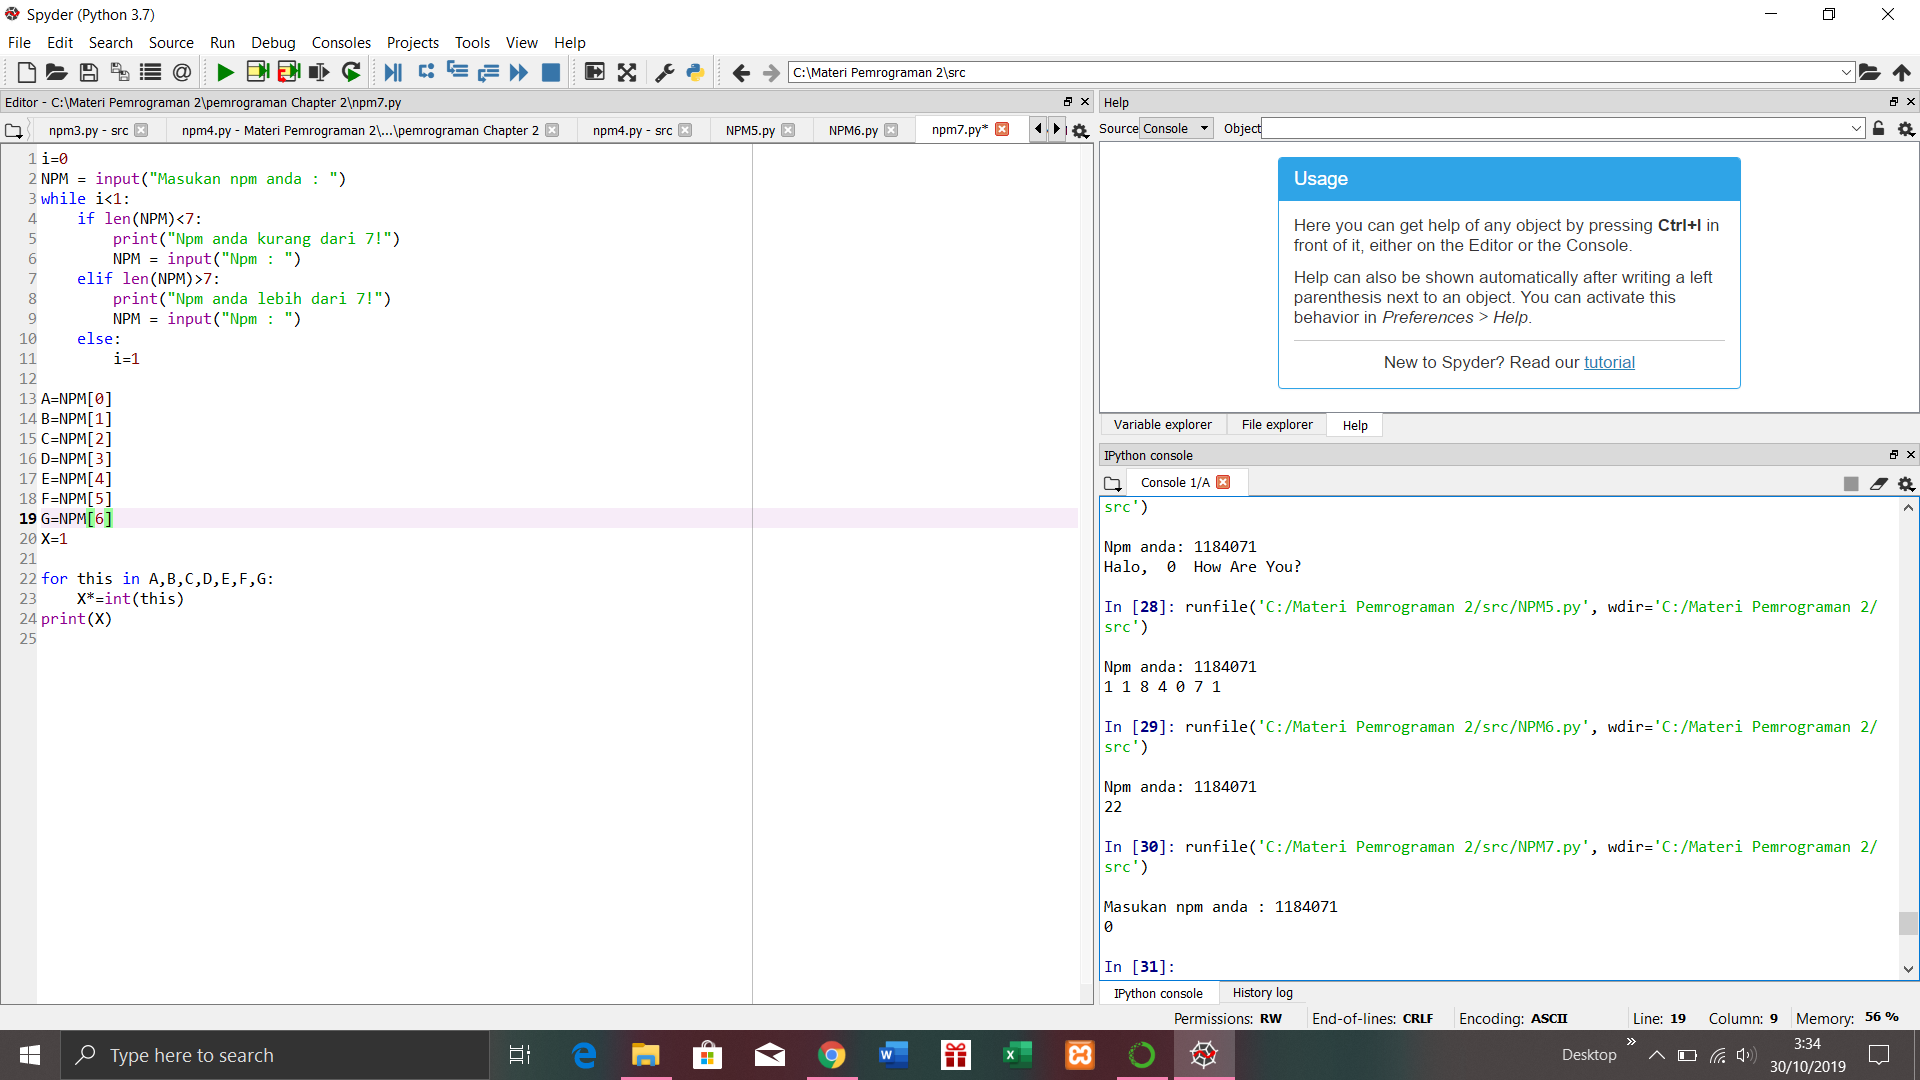
\includegraphics[width=8cm]{figures/npm7.png}}
\end{figure}
\lstinputlisting[language=Python]{figures/src/npm7.py}

\item
Dari soal no \ref{digitvar}, Lakukan print secara vertikal dari NPM anda menggunakan variabel diatas. 
\paragraph{}
\centerline{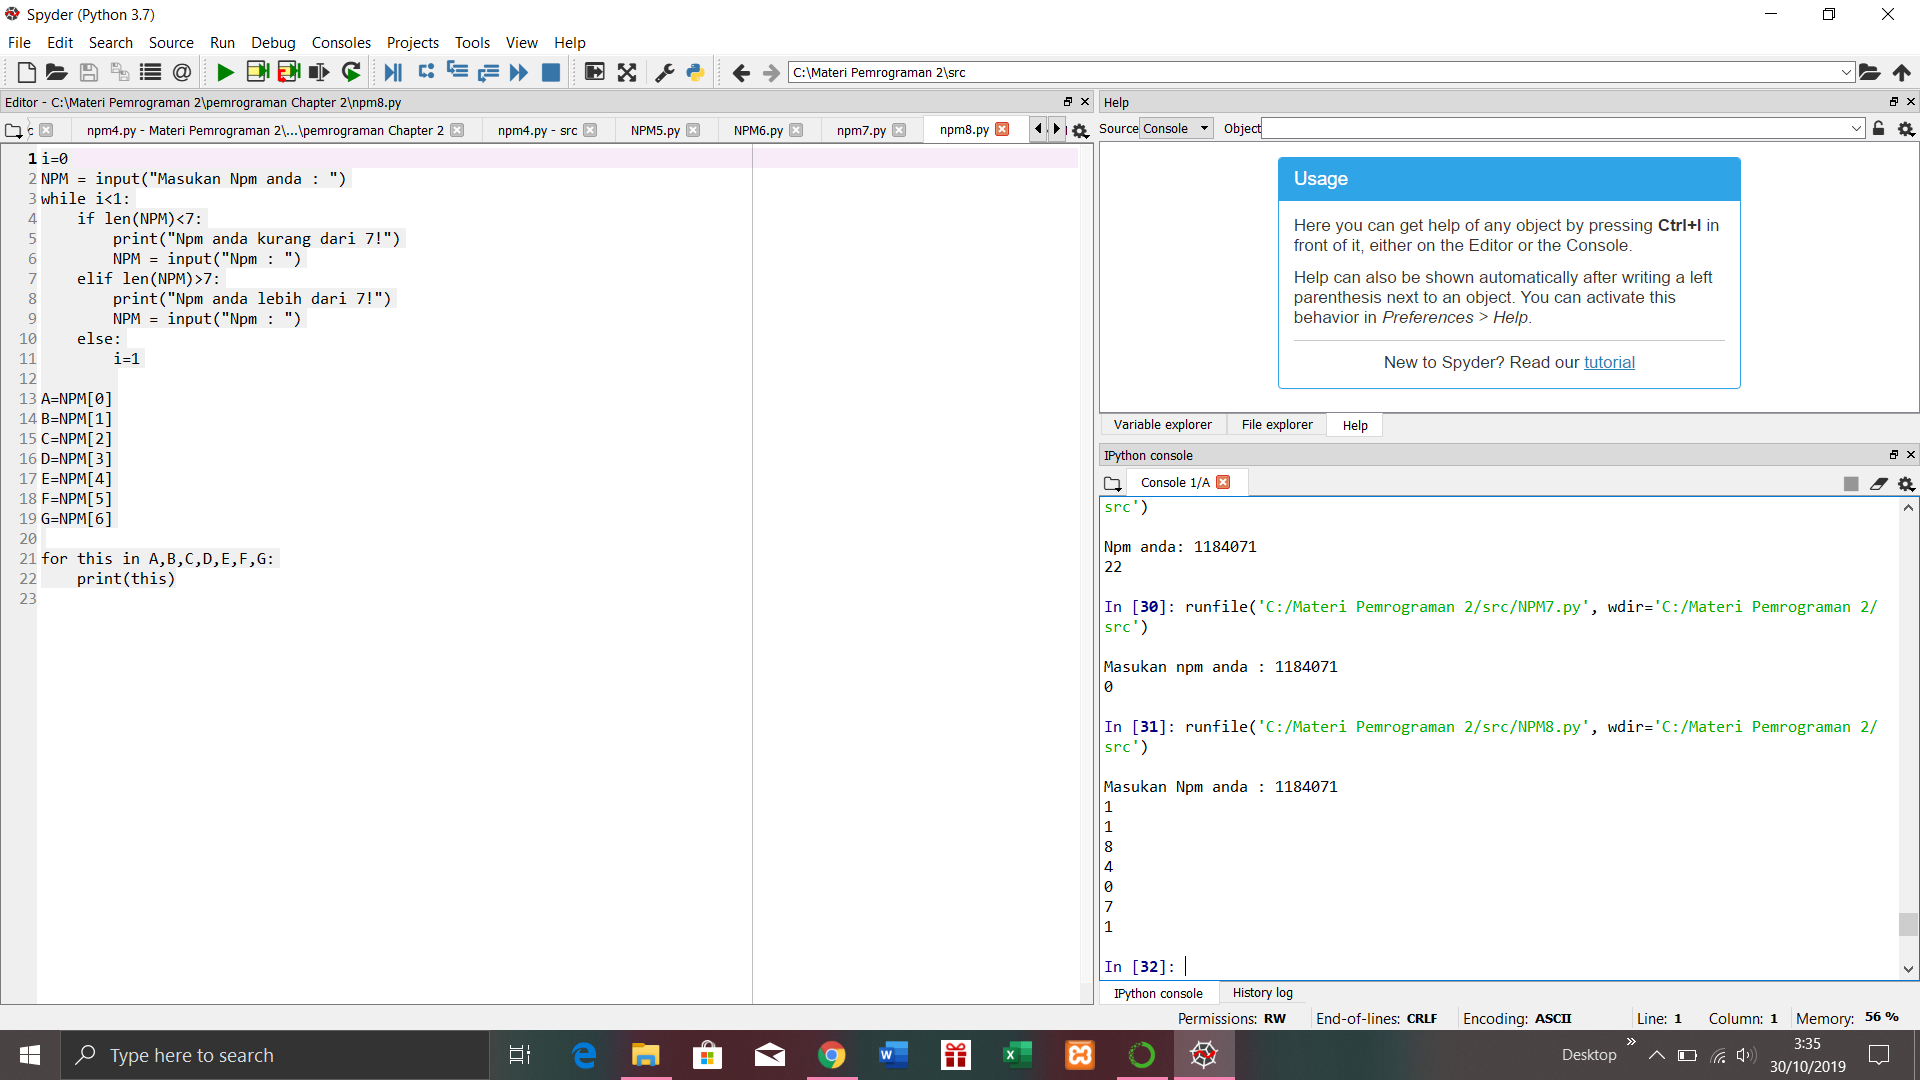
\includegraphics[width=8cm]{figures/npm8.png}}
\lstinputlisting[language=Python]{figures/src/npm8.py}

\item
Dari soal no \ref{digitvar}, Lakukan print NPM anda tapi hanya dijit genap saja. 
\begin{figure}[h]
\centerline{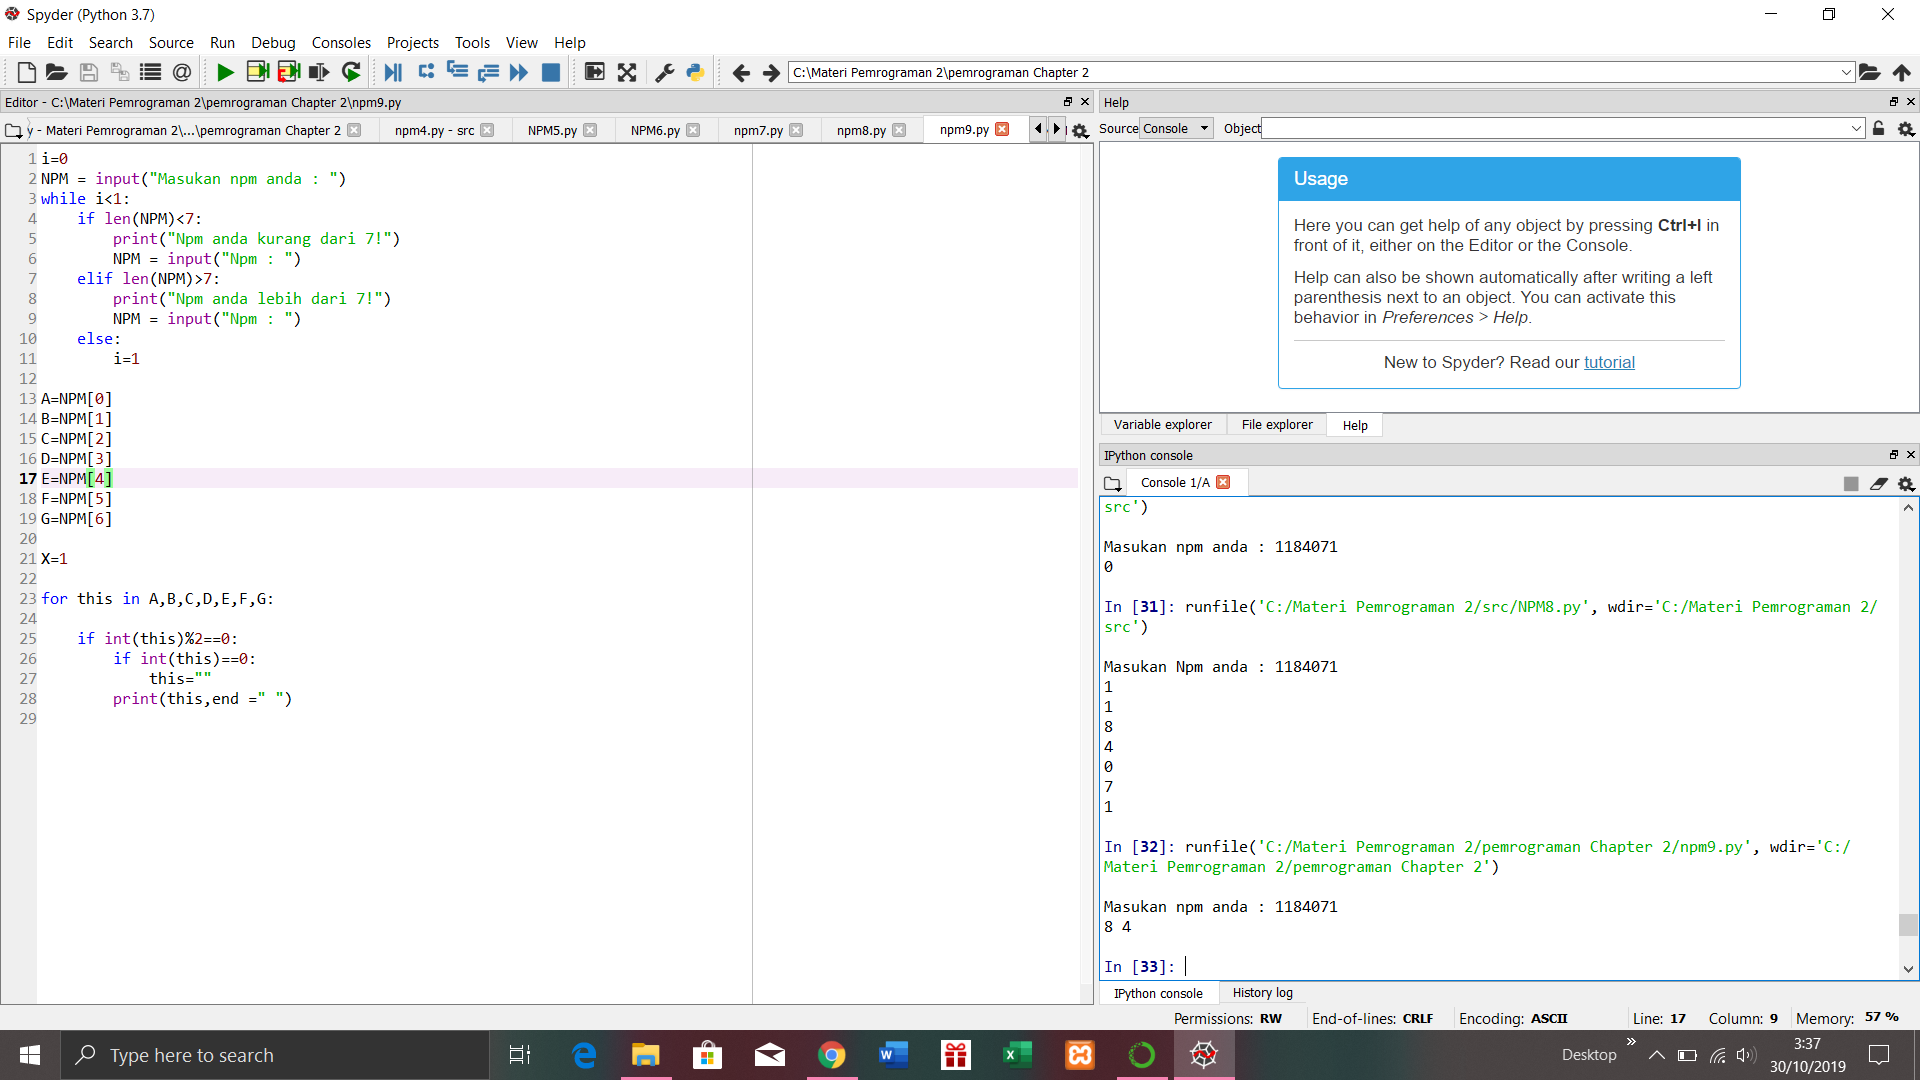
\includegraphics[width=8cm]{figures/npm9.png}}
\end{figure}
\lstinputlisting[language=Python]{figures/src/npm9.py}

\item
Dari soal no \ref{digitvar}, Lakukan print NPM anda tapi hanya dijit ganjil saja.
\begin{figure}[h]
\centerline{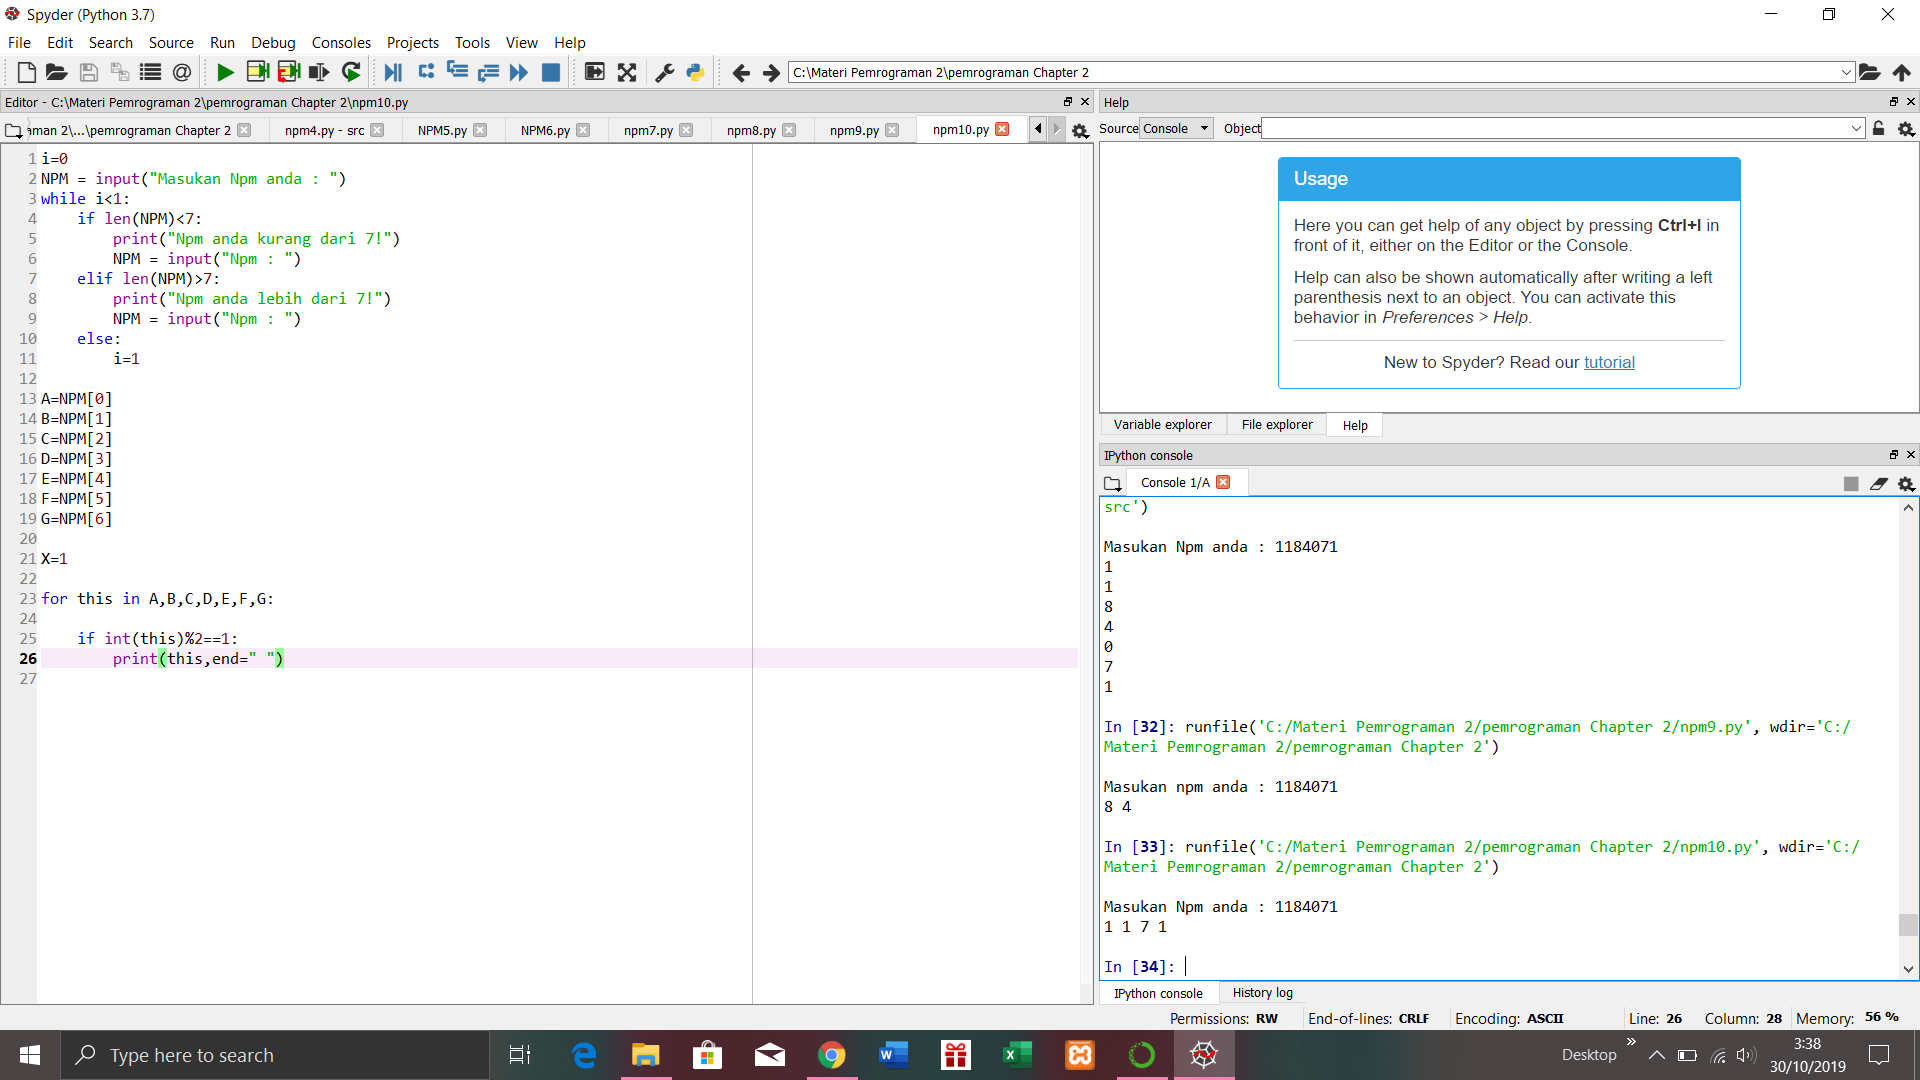
\includegraphics[width=8cm]{figures/npm10.png}}
\end{figure}
\lstinputlisting[language=Python]{figures/src/npm10.py}

\item 
Dari soal no \ref{digitvar}, Lakukan print NPM anda tapi hanya dijit yang termasuk bilangan prima saja.
\begin{figure}[h]
\centerline{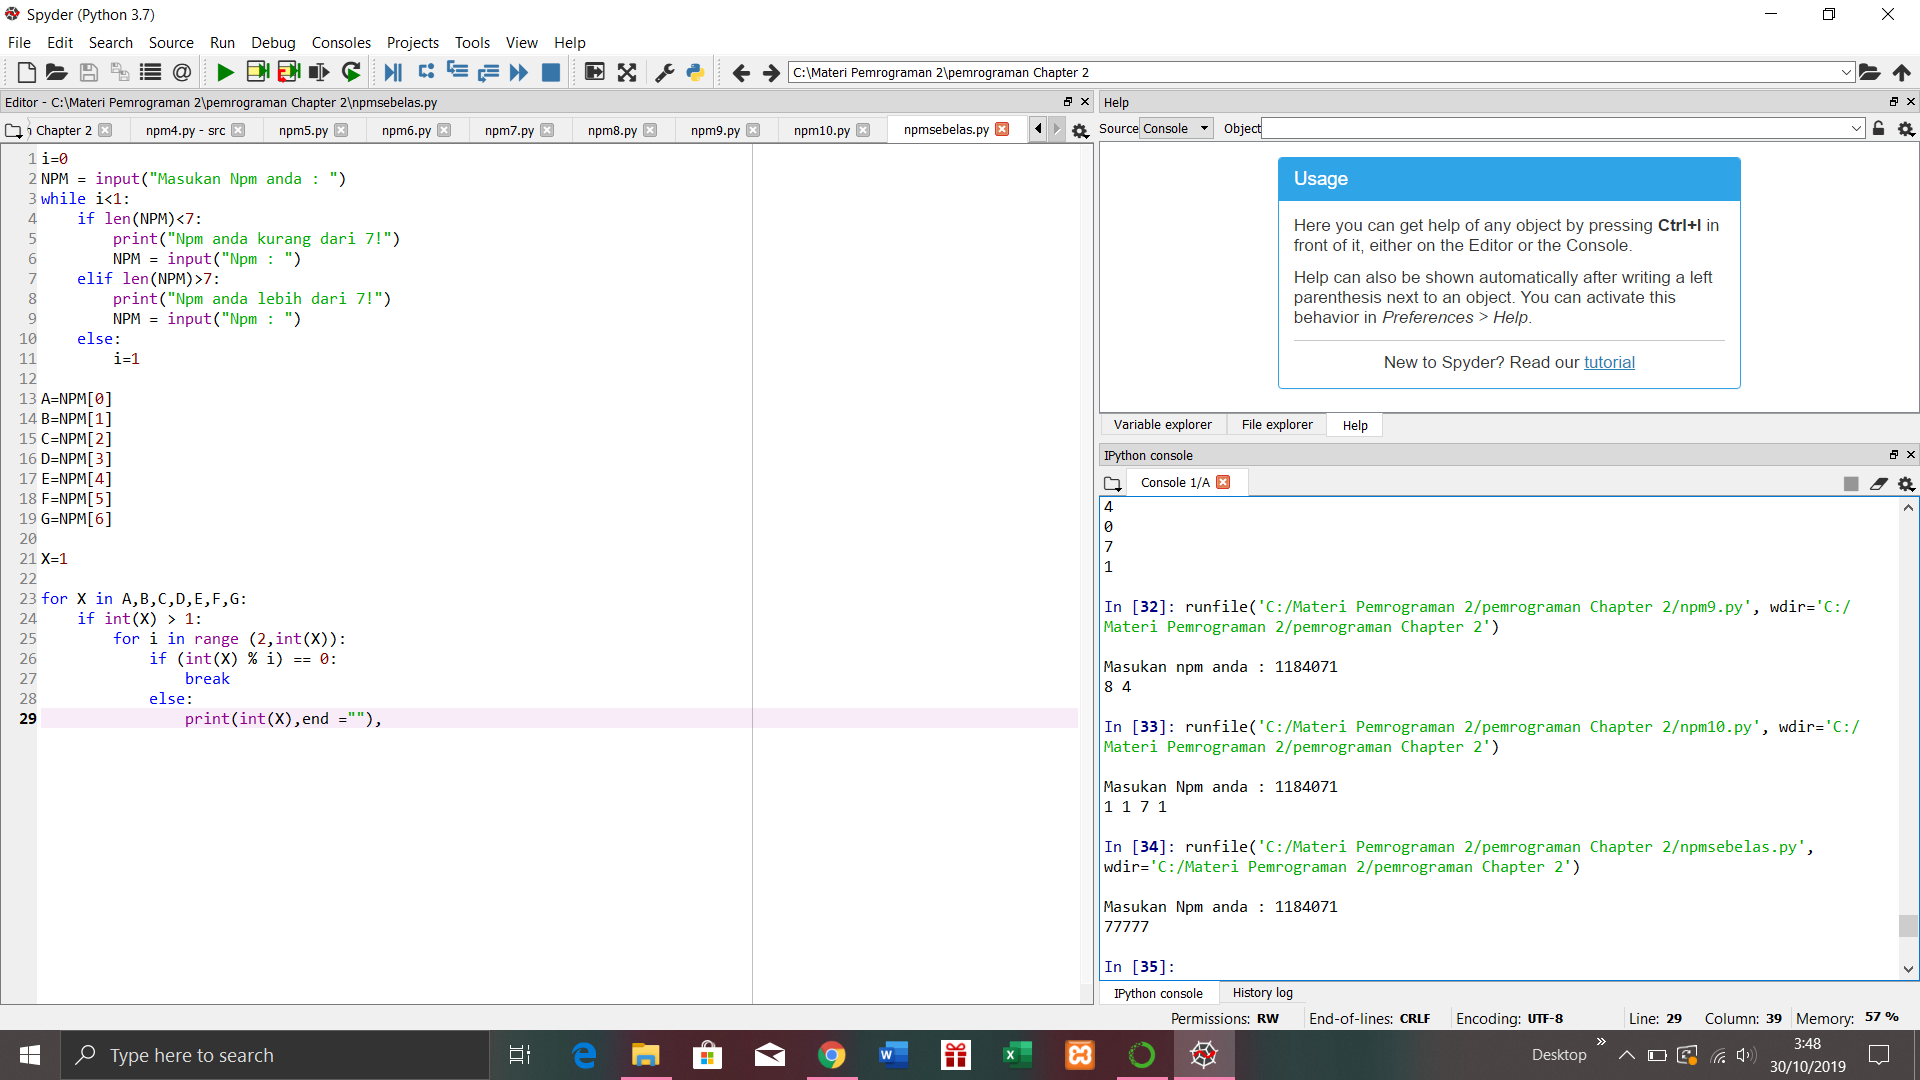
\includegraphics[width=8cm]{figures/npmsebelas.png}}
\end{figure}
\lstinputlisting[language=Python]{figures/src/npmsebelas.py}

\end{enumerate}

\section{Keterampilan Penanganan Error}
Bagian Penanganan error dari script python.
\begin{enumerate}
\item
Tuliskan peringatan error yang didapat dari mengerjakan praktek kedua ini, dan jelaskan cara penanganan error tersebut.
\par Peringatan error yang didapat adalah seperti berikut, dijelaskan bahwa penggunaan persen d untuk integer dan bukan string. Tetapi tipe data yang dimasukkan atau diinputkan adalah string, maka terjadi error.
\begin{figure}[h]
\centerline{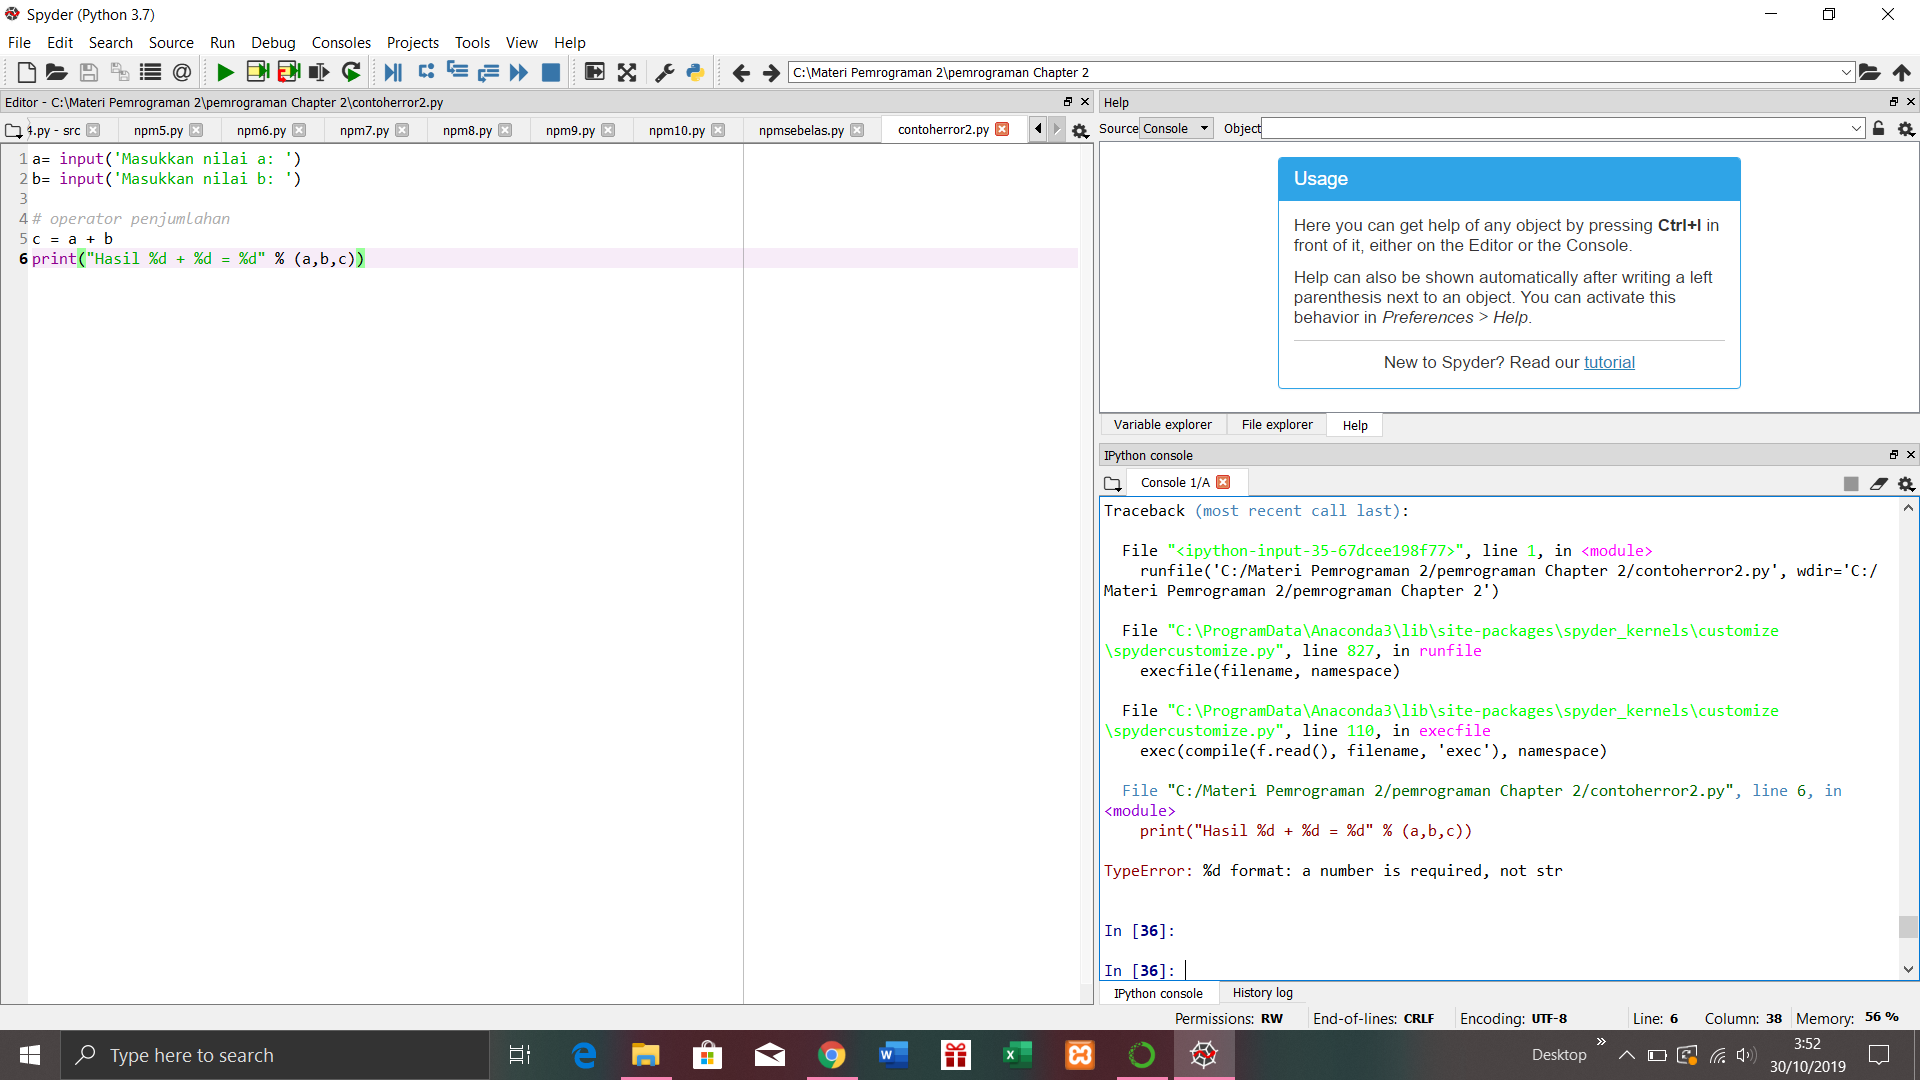
\includegraphics[width=8cm]{figures/contoherror2.png}}
\end{figure}
\lstinputlisting[language=Python]{figures/src/contoherror2.py}
\par Error akan diatasi oleh try except, dengan cara menangkap error lalu memprint peringatan error tersebut.
\paragraph{}
\centerline{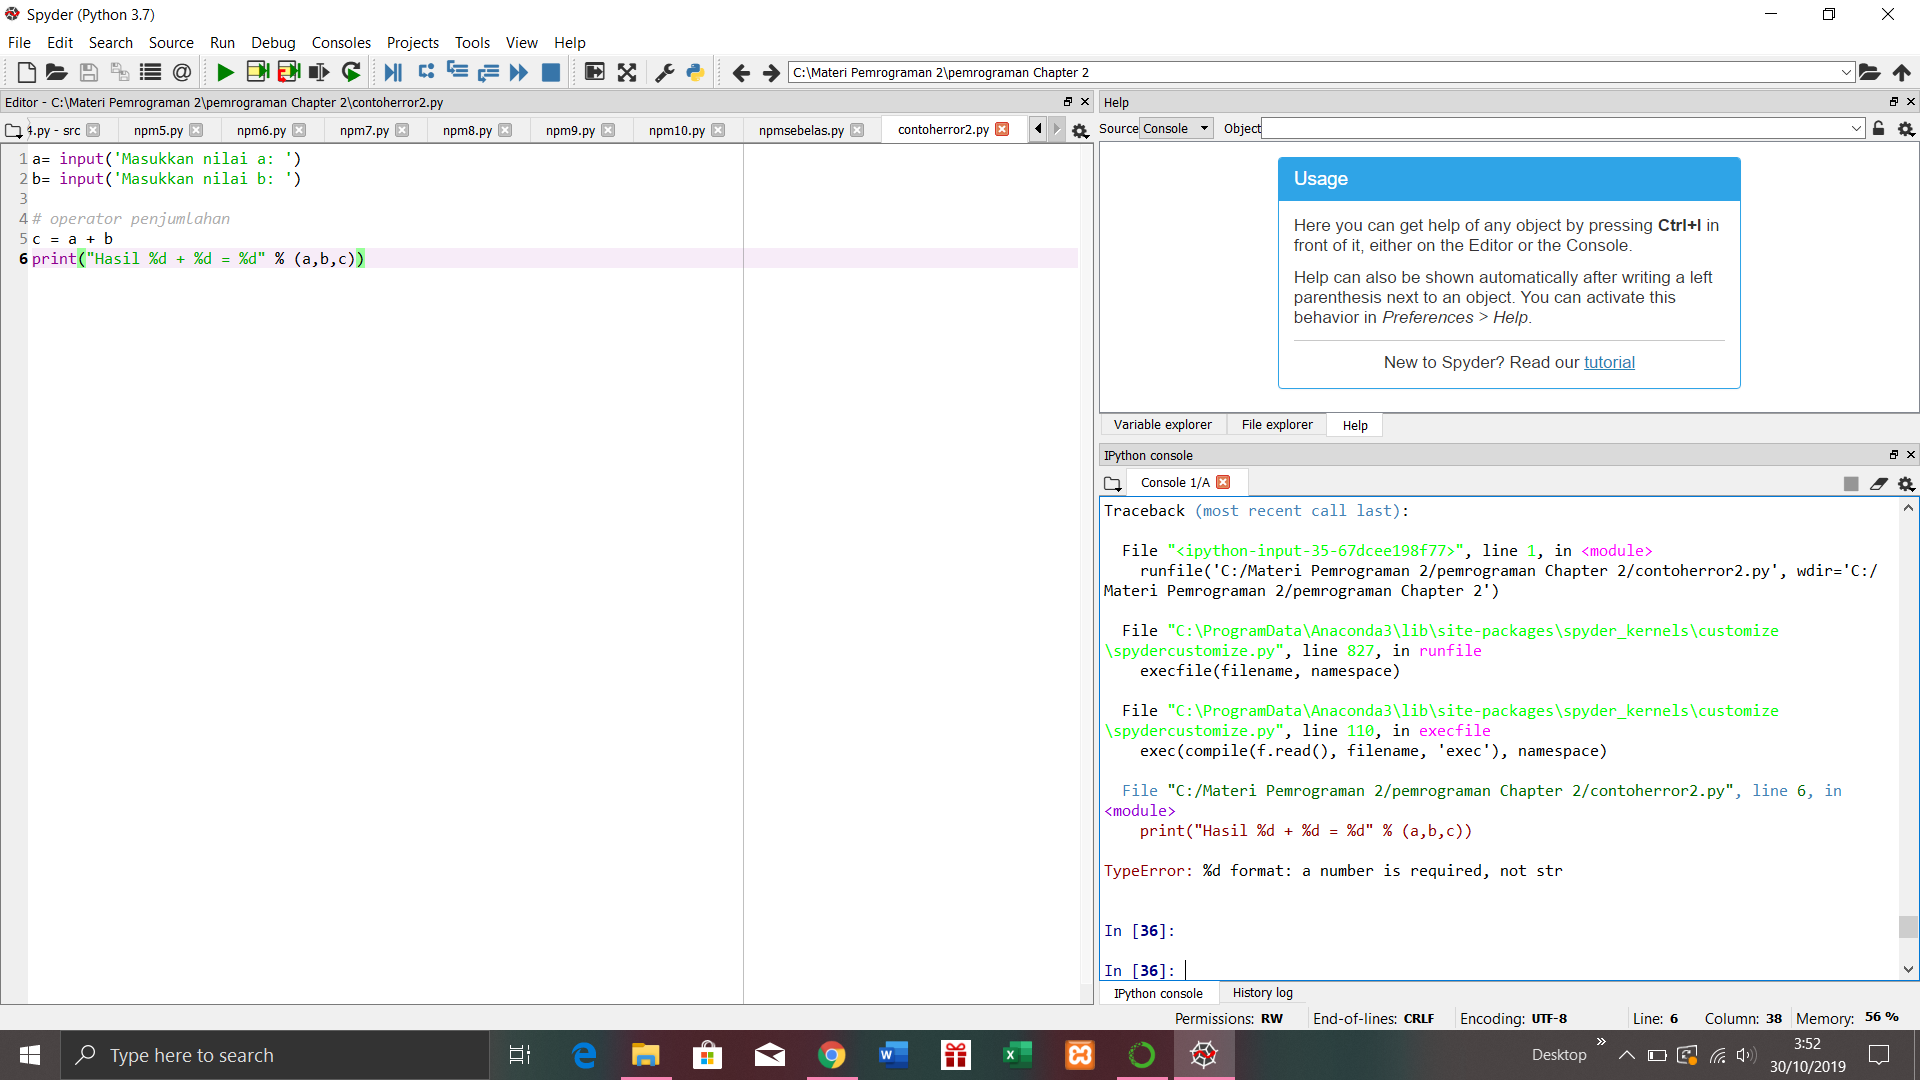
\includegraphics[width=8cm]{figures/contoherror2.png}}
\lstinputlisting[language=Python]{figures/src/contoherror.py}

\item
Membuat file 2err.py dan mengisinya dengan script pengisian variabel sebagai string dan pengisian variabel sebagai interger. 
Kemudian jumlahkan antara variabel integer dan string dan tangkap jenis errornya, gunakan try except untuk menunjukkan error tersebut dengan
bahasa indonesia.
\begin{figure}[h]
\centerline{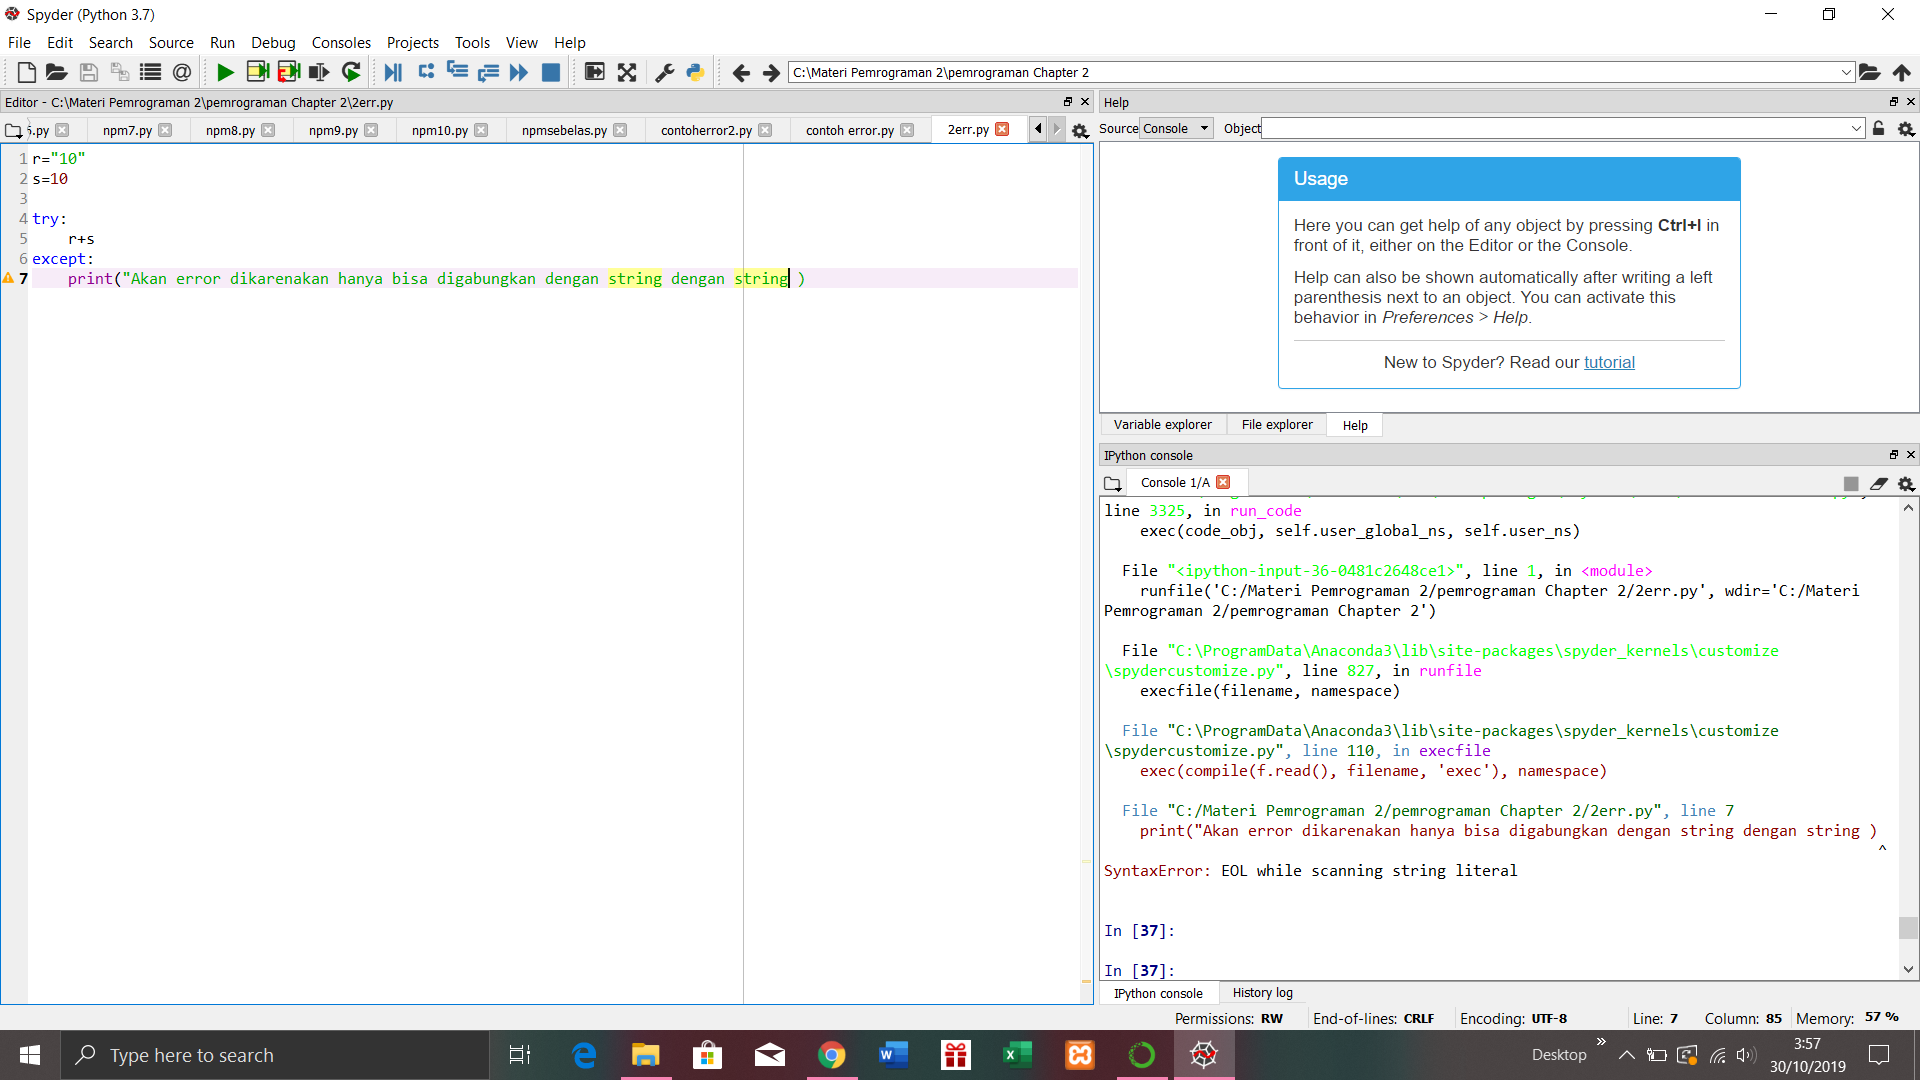
\includegraphics[width=8cm]{figures/2err.png}}
\end{figure}
\lstinputlisting[language=Python]{figures/src/2err.py} 
\end{document}
